% ============================================================
%  Network Security -- Module 8: Public Key Cryptography
%  Lesson 11: Public Key Cryptography
%  Lesson 17: RSA and Diffie-Hellman Algorithms
%  Lesson 19: Elliptic Curve Cryptography
%  Beamer (Madrid theme). Compile with: pdflatex module8.tex (twice)
% ============================================================
\documentclass[aspectratio=169,11pt,xcolor={table}]{beamer}
\usetheme{Madrid}
\usefonttheme{professionalfonts}

\usepackage[T1]{fontenc}
\usepackage{lmodern}
\usepackage{booktabs}
\usepackage{array}
\usepackage{tikz}
\usetikzlibrary{arrows.meta,positioning,shapes.geometric,shapes.symbols,
  shapes.misc,shadows,calc,fit,backgrounds,mindmap,decorations.pathmorphing,decorations.pathreplacing}

% ------------------------------------------------------------
%  Colour palette
% ------------------------------------------------------------
\definecolor{navy}{RGB}{21,45,99}
\definecolor{ocean}{RGB}{28,97,158}
\definecolor{aqua}{RGB}{0,142,150}
\definecolor{brick}{RGB}{200,55,45}
\definecolor{amber}{RGB}{235,150,20}
\definecolor{leaf}{RGB}{40,160,90}
\definecolor{grape}{RGB}{125,70,165}
\definecolor{sky}{RGB}{235,243,252}
\definecolor{ink}{RGB}{40,40,50}

\setbeamercolor{palette primary}{bg=ocean,fg=white}
\setbeamercolor{palette secondary}{bg=navy!85,fg=white}
\setbeamercolor{palette tertiary}{bg=navy,fg=white}
\setbeamercolor{palette quaternary}{bg=navy,fg=white}
\setbeamercolor{structure}{fg=ocean}
\setbeamercolor{title}{bg=navy,fg=white}
\setbeamercolor{frametitle}{bg=navy,fg=white}
\setbeamercolor{block title}{bg=ocean,fg=white}
\setbeamercolor{block body}{bg=sky,fg=ink}
\setbeamercolor{block title alerted}{bg=brick,fg=white}
\setbeamercolor{block body alerted}{bg=brick!8,fg=ink}
\setbeamercolor{block title example}{bg=leaf,fg=white}
\setbeamercolor{block body example}{bg=leaf!8,fg=ink}
\setbeamercolor{normal text}{fg=ink}
\setbeamercolor{alerted text}{fg=brick}
\setbeamercolor{item projected}{bg=ocean,fg=white}
\setbeamertemplate{items}[circle]
\setbeamertemplate{blocks}[rounded][shadow=true]
\setbeamertemplate{navigation symbols}{}

% Section divider slide
\AtBeginSection[]{
  \begin{frame}[plain]
    \begin{tikzpicture}[remember picture,overlay]
      \fill[navy] (current page.south west) rectangle (current page.north east);
      \fill[ocean] (current page.south west) rectangle ([yshift=1.2cm]current page.south east);
      \fill[aqua] ([yshift=1.2cm]current page.south west) rectangle ([yshift=1.35cm]current page.south east);
      \foreach \i in {1,...,6}
        \draw[white,opacity=0.06,line width=14pt]
          ([xshift=\i*1.6cm]current page.north west) circle (\i*0.9cm);
      \node[white,font=\large,anchor=west] at ([xshift=1.2cm,yshift=0.9cm]current page.west)
        {Lesson \thesection};
      \node[white,font=\huge\bfseries,anchor=west,text width=12cm] at ([xshift=1.2cm,yshift=-0.1cm]current page.west)
        {\insertsectionhead};
      \node[white,opacity=0.8,anchor=east,font=\small] at ([xshift=-0.8cm,yshift=0.6cm]current page.south east)
        {Module 8 \,$\cdot$\, Public Key Cryptography};
    \end{tikzpicture}
  \end{frame}
}

% ------------------------------------------------------------
%  TikZ styles and small pictograms
% ------------------------------------------------------------
\tikzset{
  >={Stealth[length=2.6mm]},
  box/.style={draw=#1!80!black,fill=#1!15,rounded corners=4pt,thick,
    minimum height=8mm,minimum width=22mm,align=center,font=\small,
    drop shadow={opacity=0.25}},
  box/.default=ocean,
  lay/.style={fill=#1,text=white,rounded corners=3pt,minimum width=38mm,minimum height=9mm,font=\scriptsize,align=center},
  solid box/.style={fill=#1,text=white,rounded corners=4pt,
    minimum height=8mm,minimum width=22mm,align=center,font=\small\bfseries,
    drop shadow={opacity=0.3}},
  solid box/.default=ocean,
  flow/.style={->,very thick,draw=#1},
  flow/.default=ink!70,
  station/.style={circle,draw=#1!80!black,fill=#1!20,very thick,minimum size=13mm,
    font=\small\bfseries,align=center},
  station/.default=ocean,
  tag/.style={font=\scriptsize,text=ink!80,align=center},
  layer/.style={draw=white,thick,fill=#1,text=white,minimum width=40mm,
    minimum height=6.5mm,font=\small\bfseries},
  % pictograms
  pics/pc/.style={code={
    \fill[#1!85!black,rounded corners=1.5pt] (-0.42,-0.05) rectangle (0.42,0.52);
    \fill[white!90!#1] (-0.36,0.01) rectangle (0.36,0.46);
    \fill[#1!85!black] (-0.06,-0.05) rectangle (0.06,-0.18);
    \fill[#1!85!black,rounded corners=1pt] (-0.24,-0.18) rectangle (0.24,-0.24);
  }},
  pics/pc/.default=ocean,
  pics/person/.style={code={
    \fill[#1] (0,0.46) circle (0.16);
    \fill[#1,rounded corners=5pt] (-0.27,-0.1) -- (-0.27,0.2) -- (0.27,0.2) -- (0.27,-0.1) -- cycle;
  }},
  pics/person/.default=ocean,
  pics/lock/.style={code={
    \draw[#1!80!black,line width=2.2pt] (-0.15,0.12) -- (-0.15,0.28) arc (180:0:0.15) -- (0.15,0.12);
    \fill[#1,rounded corners=2pt] (-0.26,-0.22) rectangle (0.26,0.14);
    \fill[white] (0,-0.02) circle (0.05);
    \fill[white] (-0.02,-0.02) rectangle (0.02,-0.13);
  }},
  pics/lock/.default=amber,
  pics/doc/.style={code={
    \fill[white,draw=#1,thick] (-0.25,-0.33) -- (-0.25,0.33) -- (0.12,0.33) -- (0.25,0.2) -- (0.25,-0.33) -- cycle;
    \draw[#1,thick] (0.12,0.33) -- (0.12,0.2) -- (0.25,0.2);
    \foreach \y in {0.12,0,-0.12,-0.24} \draw[#1!70,thick] (-0.16,\y) -- (0.16,\y);
  }},
  pics/doc/.default=ocean,
  pics/key/.style={code={
    \draw[#1,line width=2pt] (0,0) circle (0.12);
    \draw[#1,line width=2pt] (0.12,0) -- (0.5,0) (0.38,0) -- (0.38,-0.12) (0.47,0) -- (0.47,-0.1);
  }},
  pics/key/.default=amber,
}
\newcommand{\comma}{,}
\newcommand{\hl}[1]{\textcolor{ocean}{\textbf{#1}}}
\newcommand{\bad}[1]{\textcolor{brick}{\textbf{#1}}}
\newcommand{\good}[1]{\textcolor{leaf}{\textbf{#1}}}

\makeatletter
% University logo, small, top-right corner of every page
\AddToHook{shipout/foreground}{%
  \put(\strip@pt\paperwidth,0){%
    \makebox(0,0)[tr]{\raisebox{-0.8cm}{
\includegraphics[height=0.72cm]{au_logo.png}\hspace{0.15cm}}}}}
\makeatother

% ------------------------------------------------------------
\title[Module 8: Public Key Cryptography]{Public Key Cryptography}
\subtitle{Module 8 \,\textbar\, Lesson 11: Public Key Cryptography \,\textbullet\, Lesson 17: RSA and Diffie--Hellman \,\textbullet\, Lesson 19: Elliptic Curve Cryptography}
\author[Network Security]{Network Security}
\institute[SLM]{Self-Learning Material \,--\, Lessons 11, 17 \& 19}
\date{}

\newcommand{\qa}[3]{%
  \node[circle,fill=#3,text=white,font=\bfseries,minimum size=8mm] at (0,#1) {Q};
}

\begin{document}

% ============================================================
\begin{frame}[plain]
  
\begin{tikzpicture}[remember picture,overlay]
    \shade[top color=navy,bottom color=ocean] (current page.south west) rectangle (current page.north east);
    \foreach \i/\o in {1/0.10,2/0.08,3/0.06,4/0.05,5/0.04}
      \draw[white,opacity=\o,line width=1.2pt] ([xshift=-2.5cm,yshift=-0.5cm]current page.north east) circle (\i*1.1cm);
    \fill[aqua] ([yshift=2.35cm]current page.south west) rectangle ([yshift=2.45cm]current page.south east);
    \begin{scope}[shift={([xshift=-3.0cm,yshift=0.5cm]current page.east)}]
      \fill[white,opacity=0.15] (0,0) circle (1.7);
      \pic[scale=1.9] at (-0.75,0.55) {key=leaf};
      \pic[scale=1.9] at (-0.75,-0.55) {key=brick};
      \node[white,font=\scriptsize\bfseries] at (0.95,0.55) {public};
      \node[white,font=\scriptsize\bfseries] at (0.95,-0.55) {private};
    \end{scope}
    \node[white,anchor=west,font=\normalsize] at ([xshift=1.1cm,yshift=2.4cm]current page.west)
      {NETWORK SECURITY \,\textbar\, MODULE 8};
    \node[white,anchor=west,font=\fontsize{28}{33}\selectfont\bfseries,text width=10cm] at ([xshift=1.1cm,yshift=1.0cm]current page.west)
      {Public Key\\[2pt] Cryptography};
    \node[white,opacity=0.9,anchor=west,text width=9.5cm,font=\small] at ([xshift=1.1cm,yshift=-0.95cm]current page.west)
      {Lesson 11 \,--\, Public Key Cryptography\\ Lesson 17 \,--\, RSA and Diffie--Hellman Algorithms\\ Lesson 19 \,--\, Elliptic Curve Cryptography};
    \node[white,opacity=0.85,anchor=west,font=\footnotesize] at ([xshift=1.1cm,yshift=1.2cm]current page.south west)
      {Key pairs \,$\cdot$\, Trap-door functions \,$\cdot$\, RSA \,$\cdot$\, Square-and-multiply \,$\cdot$\, CRT \,$\cdot$\, Diffie--Hellman \,$\cdot$\, MITM \,$\cdot$\, ECC};
  \end{tikzpicture}
\end{frame}

% ============================================================
\begin{frame}{Roadmap of This Module}
  \centering
  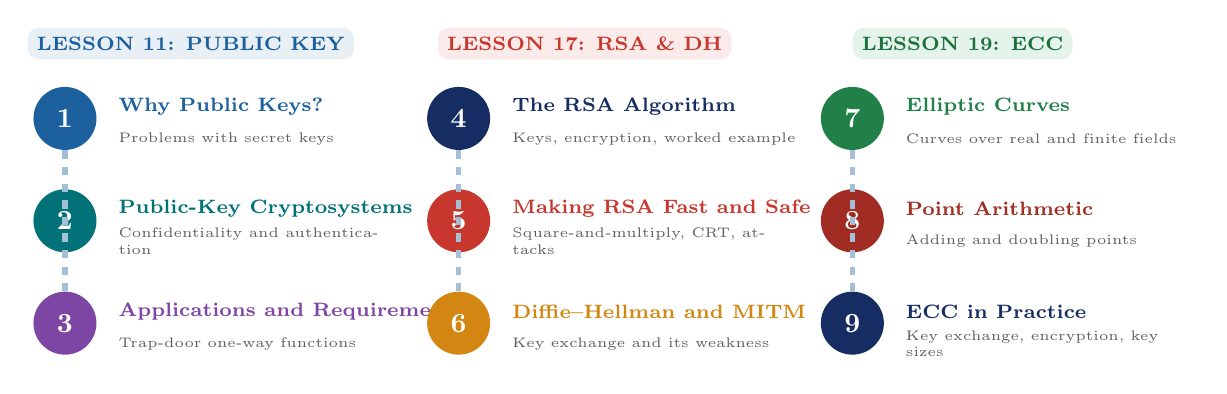
\begin{tikzpicture}
    \foreach \t/\c/\n/\x/\y [count=\i] in {
      Why Public Keys?/ocean/Problems with secret keys/0/0,
      Public-Key Cryptosystems/aqua!80!black/Confidentiality and authentication/0/-1.3,
      Applications and Requirements/grape/Trap-door one-way functions/0/-2.6,
      The RSA Algorithm/navy/Keys\comma{} encryption\comma{} worked example/5.0/0,
      Making RSA Fast and Safe/brick/Square-and-multiply\comma{} CRT\comma{} attacks/5.0/-1.3,
      Diffie--Hellman and MITM/amber!90!black/Key exchange and its weakness/5.0/-2.6,
      Elliptic Curves/leaf!80!black/Curves over real and finite fields/10.0/0,
      Point Arithmetic/brick!80!black/Adding and doubling points/10.0/-1.3,
      ECC in Practice/navy/Key exchange\comma{} encryption\comma{} key sizes/10.0/-2.6}
    {
      \node[circle,fill=\c,text=white,font=\bfseries,minimum size=8mm] (n\i) at (\x,\y) {\i};
      \node[anchor=west,font=\scriptsize\bfseries,text=\c] at ([xshift=1.5mm,yshift=1.5mm]n\i.east) {\t};
      \node[anchor=west,font=\tiny,text=ink!75,text width=36mm] at ([xshift=1.5mm,yshift=-2.6mm]n\i.east) {\n};
    }
    \draw[ocean!40,line width=2pt,dashed] (n1) -- (n3);
    \draw[ocean!40,line width=2pt,dashed] (n4) -- (n6);
    \draw[ocean!40,line width=2pt,dashed] (n7) -- (n9);
    \node[fill=ocean!10,rounded corners,font=\scriptsize\bfseries,text=ocean] at (1.6,0.95) {LESSON 11: PUBLIC KEY};
    \node[fill=brick!10,rounded corners,font=\scriptsize\bfseries,text=brick] at (6.6,0.95) {LESSON 17: RSA \& DH};
    \node[fill=leaf!12,rounded corners,font=\scriptsize\bfseries,text=leaf!70!black] at (11.4,0.95) {LESSON 19: ECC};
  \end{tikzpicture}
\end{frame}

% ============================================================
\setcounter{section}{10}
\section{Public Key Cryptography}
% ============================================================

\begin{frame}{Why Do We Need Public Keys?}
  \begin{columns}[c]
    \begin{column}{0.5\textwidth}
      \centering
      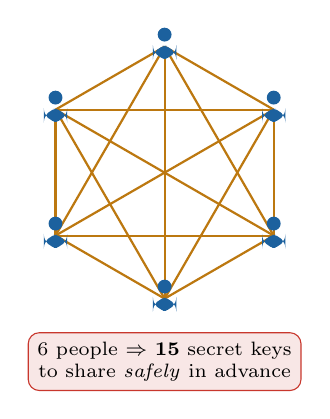
\begin{tikzpicture}
        \foreach \a [count=\i] in {90,150,210,270,330,30}
          \coordinate (p\i) at (\a:1.6);
        \foreach \i in {1,...,6} \foreach \j in {1,...,6} {\ifnum\i<\j \draw[amber!80!black,thick] (p\i) -- (p\j);\fi}
        \foreach \i in {1,...,6} \pic[scale=0.55] at ($(p\i)+(0,-0.1)$) {person=ocean};
        \node[fill=brick!12,draw=brick,rounded corners,font=\scriptsize,align=center] at (0,-2.4) {6 people $\Rightarrow$ \textbf{15} secret keys\\to share \emph{safely} in advance};
      \end{tikzpicture}
    \end{column}
    \begin{column}{0.48\textwidth}
      {\small Secret-key (symmetric) cryptography left two problems unsolved:}
      \begin{alertblock}{1. Key distribution}
        \small How do two strangers agree on a shared key \textbf{without} meeting first, and without trusting a KDC?
      \end{alertblock}
      \begin{alertblock}{2. Digital signatures}
        \small How can a message prove \textbf{who wrote it}, the way a handwritten signature does?
      \end{alertblock}
      \begin{exampleblock}{The breakthrough}
        \small \textbf{Diffie and Hellman, 1976}: use \textbf{two different keys}, one public and one private.
      \end{exampleblock}
    \end{column}
  \end{columns}
\end{frame}

% ------------------------------------------------------------
\begin{frame}{Three Common Misconceptions}
  \centering
  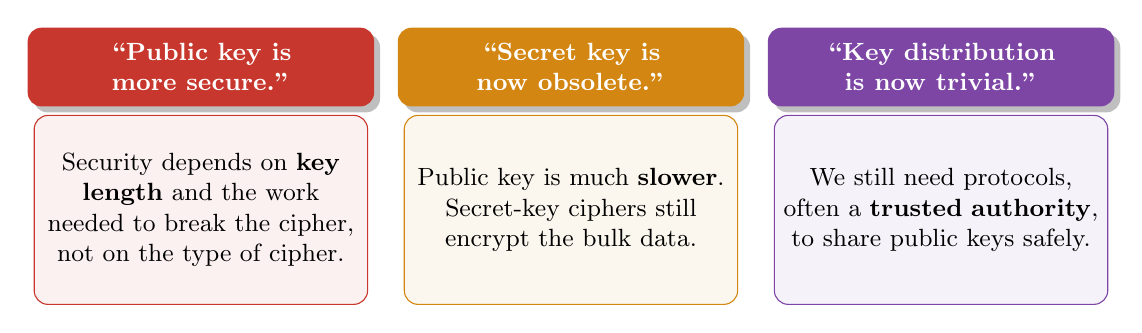
\begin{tikzpicture}
    \foreach \x/\c/\m/\t in {
      0/brick/``Public key is more secure.''/Security depends on \textbf{key length} and the work needed to break the cipher\comma{} not on the type of cipher.,
      4.7/amber!90!black/``Secret key is now obsolete.''/Public key is much \textbf{slower}. Secret-key ciphers still encrypt the bulk data.,
      9.4/grape/``Key distribution is now trivial.''/We still need protocols\comma{} often a \textbf{trusted authority}\comma{} to share public keys safely.}
    {
      \node[fill=\c,text=white,rounded corners=5pt,font=\small\bfseries,minimum width=44mm,minimum height=10mm,text width=41mm,align=center,drop shadow] (h) at (\x,0) {\m};
      \node[draw=\c,fill=\c!7,rounded corners=5pt,text width=40mm,minimum height=24mm,font=\small,anchor=north,align=center] at ([yshift=-1mm]h.south) {\t};
    }
  \end{tikzpicture}
  \vspace{3mm}
  \begin{block}{In practice}
    \small Public-key and secret-key cryptography \textbf{work together}: public key to exchange a session key, secret key to encrypt the data.
  \end{block}
\end{frame}

% ------------------------------------------------------------
\begin{frame}{Ingredients of a Public-Key Cryptosystem}
  \begin{columns}[c]
    \begin{column}{0.48\textwidth}
      \centering
      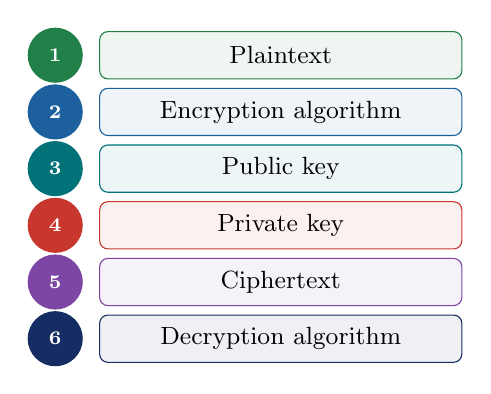
\begin{tikzpicture}
        \foreach \t/\c [count=\i from 0] in {Plaintext/leaf!80!black,Encryption algorithm/ocean,Public key/aqua!80!black,Private key/brick,Ciphertext/grape,Decryption algorithm/navy}{
          \node[circle,fill=\c,text=white,font=\scriptsize\bfseries,minimum size=7mm] (c\i) at (0,-\i*0.72) {\the\numexpr\i+1\relax};
          \node[draw=\c,fill=\c!7,rounded corners=3pt,anchor=west,minimum width=46mm,minimum height=6mm,font=\small] at ([xshift=2mm]c\i.east) {\t};
        }
      \end{tikzpicture}
    \end{column}
    \begin{column}{0.5\textwidth}
      \begin{block}{The key pair}
        \small Each user generates a \textbf{pair} of related keys:
        \begin{itemize}\setlength{\itemsep}{1pt}
          \item the \textbf{public key} $PU$: published for everyone
          \item the \textbf{private key} $PR$: kept secret by the owner
        \end{itemize}
      \end{block}
      \begin{exampleblock}{Golden rule}
        \small What one key locks, \textbf{only the other key} of the same pair can unlock.
      \end{exampleblock}
      {\small Also called \textbf{asymmetric} cryptography, because the two keys are different.}
    \end{column}
  \end{columns}
\end{frame}

% ------------------------------------------------------------
\begin{frame}{Encryption with the Public Key: Confidentiality}
  \centering
  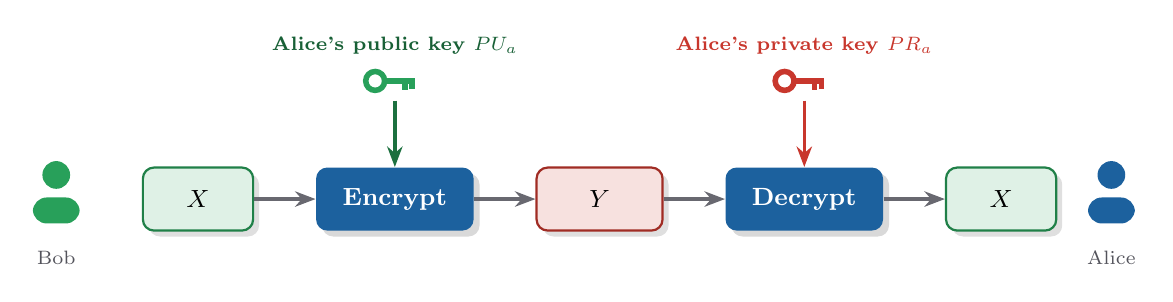
\begin{tikzpicture}
    \pic[scale=1.1] at (0,0) {person=leaf}; \node[tag] at (0,-0.55) {Bob};
    \node[box=leaf,minimum width=14mm] (x) at (1.8,0.2) {$X$};
    \node[solid box=ocean,minimum width=20mm] (e) at (4.3,0.2) {Encrypt};
    \node[box=brick,minimum width=16mm] (y) at (6.9,0.2) {$Y$};
    \node[solid box=ocean,minimum width=20mm] (d) at (9.5,0.2) {Decrypt};
    \node[box=leaf,minimum width=14mm] (x2) at (12.0,0.2) {$X$};
    \pic[scale=1.1] at (13.4,0) {person=ocean}; \node[tag] at (13.4,-0.55) {Alice};
    \draw[flow] (x) -- (e); \draw[flow] (e) -- (y); \draw[flow] (y) -- (d); \draw[flow] (d) -- (x2);
    \pic at (4.05,1.7) {key=leaf}; \node[font=\scriptsize\bfseries,text=leaf!60!black] at (4.3,2.15) {Alice's \textbf{public} key $PU_a$};
    \pic at (9.25,1.7) {key=brick}; \node[font=\scriptsize\bfseries,text=brick] at (9.5,2.15) {Alice's \textbf{private} key $PR_a$};
    \draw[->,leaf!70!black,very thick] (4.3,1.45) -- (e); \draw[->,brick,very thick] (9.5,1.45) -- (d);
  \end{tikzpicture}
  \vspace{3mm}
  \begin{columns}[T]
    \begin{column}{0.5\textwidth}
      \begin{block}{How it works}
        \small Bob encrypts with \textbf{Alice's public key}: $Y = E(PU_a, X)$. Only Alice's \textbf{private key} can decrypt: $X = D(PR_a, Y)$.
      \end{block}
    \end{column}
    \begin{column}{0.46\textwidth}
      \begin{exampleblock}{Analogy}
        \small A post-box with a slot: \textbf{anyone} can drop a letter in, but only the owner has the key to \textbf{open} it.
      \end{exampleblock}
    \end{column}
  \end{columns}
\end{frame}

% ------------------------------------------------------------
\begin{frame}{Encryption with the Private Key: Authentication}
  \centering
  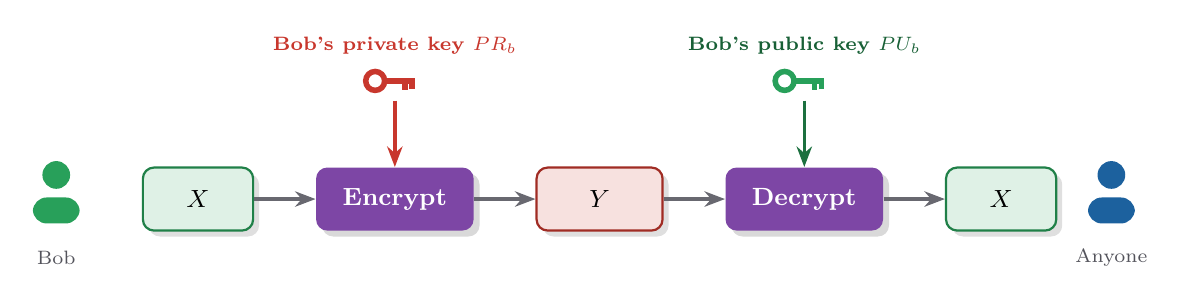
\begin{tikzpicture}
    \pic[scale=1.1] at (0,0) {person=leaf}; \node[tag] at (0,-0.55) {Bob};
    \node[box=leaf,minimum width=14mm] (x) at (1.8,0.2) {$X$};
    \node[solid box=grape,minimum width=20mm] (e) at (4.3,0.2) {Encrypt};
    \node[box=brick,minimum width=16mm] (y) at (6.9,0.2) {$Y$};
    \node[solid box=grape,minimum width=20mm] (d) at (9.5,0.2) {Decrypt};
    \node[box=leaf,minimum width=14mm] (x2) at (12.0,0.2) {$X$};
    \pic[scale=1.1] at (13.4,0) {person=ocean}; \node[tag] at (13.4,-0.55) {Anyone};
    \draw[flow] (x) -- (e); \draw[flow] (e) -- (y); \draw[flow] (y) -- (d); \draw[flow] (d) -- (x2);
    \pic at (4.05,1.7) {key=brick}; \node[font=\scriptsize\bfseries,text=brick] at (4.3,2.15) {Bob's \textbf{private} key $PR_b$};
    \pic at (9.25,1.7) {key=leaf}; \node[font=\scriptsize\bfseries,text=leaf!60!black] at (9.5,2.15) {Bob's \textbf{public} key $PU_b$};
    \draw[->,brick,very thick] (4.3,1.45) -- (e); \draw[->,leaf!70!black,very thick] (9.5,1.45) -- (d);
  \end{tikzpicture}
  \vspace{3mm}
  \begin{columns}[T]
    \begin{column}{0.5\textwidth}
      \begin{block}{How it works}
        \small Bob encrypts with his \textbf{own private key}. Anyone can decrypt with Bob's public key, so the message is \textbf{not secret}, but it \textbf{must have come from Bob}.
      \end{block}
    \end{column}
    \begin{column}{0.46\textwidth}
      \begin{exampleblock}{This is a digital signature}
        \small Gives \textbf{authentication} and \textbf{data integrity}: nobody else could have produced $Y$.
      \end{exampleblock}
    \end{column}
  \end{columns}
\end{frame}

% ------------------------------------------------------------
\begin{frame}{Secrecy and Authentication Together}
  \centering
  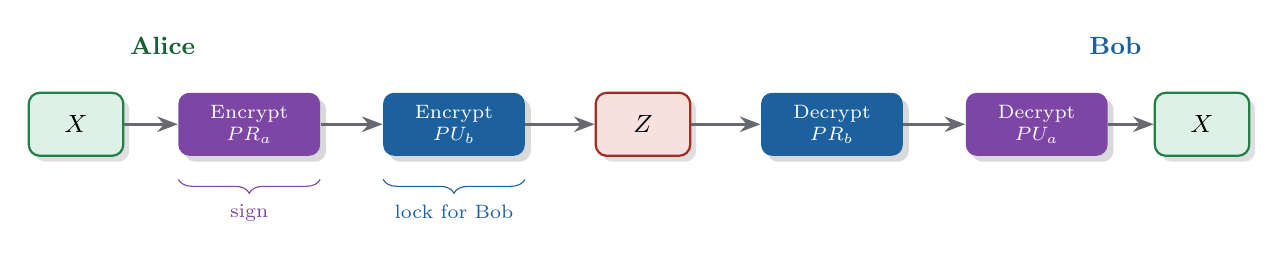
\begin{tikzpicture}
    \node[box=leaf,minimum width=12mm] (x) at (0,0) {$X$};
    \node[solid box=grape,minimum width=18mm,font=\scriptsize] (e1) at (2.2,0) {Encrypt\\$PR_a$};
    \node[solid box=ocean,minimum width=18mm,font=\scriptsize] (e2) at (4.8,0) {Encrypt\\$PU_b$};
    \node[box=brick,minimum width=12mm] (z) at (7.2,0) {$Z$};
    \node[solid box=ocean,minimum width=18mm,font=\scriptsize] (d2) at (9.6,0) {Decrypt\\$PR_b$};
    \node[solid box=grape,minimum width=18mm,font=\scriptsize] (d1) at (12.2,0) {Decrypt\\$PU_a$};
    \node[box=leaf,minimum width=12mm] (x2) at (14.3,0) {$X$};
    \foreach \a/\b in {x/e1,e1/e2,e2/z,z/d2,d2/d1,d1/x2} \draw[flow] (\a) -- (\b);
    \draw[grape,decorate,decoration={brace,amplitude=5pt,mirror}] (1.3,-0.7) -- node[below=2mm,font=\scriptsize,text=grape]{sign} (3.1,-0.7);
    \draw[ocean,decorate,decoration={brace,amplitude=5pt,mirror}] (3.9,-0.7) -- node[below=2mm,font=\scriptsize,text=ocean]{lock for Bob} (5.7,-0.7);
    \node[font=\small\bfseries,text=leaf!60!black] at (1.1,1.0) {Alice};
    \node[font=\small\bfseries,text=ocean] at (13.2,1.0) {Bob};
  \end{tikzpicture}
  \vspace{6mm}
  \begin{block}{Formula}
    \small $Z = E(PU_b,\ E(PR_a, X))$ \qquad and \qquad $X = D(PU_a,\ D(PR_b, Z))$
  \end{block}
  {\small Alice first \textbf{signs} with her private key, then \textbf{locks} the result with Bob's public key. The cost: the slow public-key algorithm is used \textbf{four times}.}
\end{frame}

% ------------------------------------------------------------
\begin{frame}{Conventional vs.\ Public-Key Encryption}
  \centering
  \renewcommand{\arraystretch}{1.4}
  \small
  \begin{tabular}{>{\bfseries}l >{\columncolor{ocean!8}\raggedright\arraybackslash}p{5cm} >{\columncolor{grape!8}\raggedright\arraybackslash}p{5cm}}
    \toprule
    \rowcolor{navy}\textcolor{white}{Feature} & \textcolor{white}{\textbf{Conventional (symmetric)}} & \textcolor{white}{\textbf{Public key (asymmetric)}}\\
    \midrule
    Keys & One key, shared by both & A pair: public + private\\
    Algorithm & Same algorithm and key both ways & One key encrypts, the other decrypts\\
    Must keep secret & The shared key & Only the private key\\
    Speed & Fast & Much slower\\
    Key distribution & Hard: needs a secure channel & Easier: public keys can be published\\
    Signatures & Not directly & Yes\\
    Examples & DES, IDEA, AES & RSA, Diffie--Hellman, ECC\\
    \bottomrule
  \end{tabular}
\end{frame}

% ------------------------------------------------------------
\begin{frame}{Applications for Public-Key Cryptosystems}
  \begin{columns}[c]
    \begin{column}{0.44\textwidth}
      \centering
      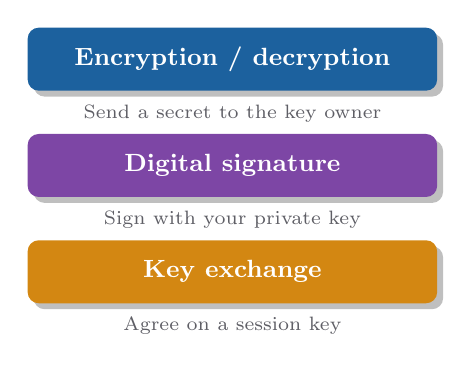
\begin{tikzpicture}
        \foreach \t/\d/\c [count=\i from 0] in {Encryption \slash{} decryption/Send a secret to the key owner/ocean,Digital signature/Sign with your private key/grape,Key exchange/Agree on a session key/amber!90!black}{
          \node[fill=\c,text=white,rounded corners=4pt,font=\small\bfseries,minimum width=52mm,minimum height=8mm,drop shadow] (h\i) at (0,-\i*1.35) {\t};
          \node[font=\scriptsize,text=ink!75,below=0.5mm of h\i] {\d};
        }
      \end{tikzpicture}
    \end{column}
    \begin{column}{0.54\textwidth}
      \centering
      \renewcommand{\arraystretch}{1.35}
      \small
      \begin{tabular}{l c c c}
        \toprule
        \rowcolor{navy}\textcolor{white}{\textbf{Algorithm}} & \textcolor{white}{\textbf{Enc/Dec}} & \textcolor{white}{\textbf{Signature}} & \textcolor{white}{\textbf{Key exch.}}\\
        \midrule
        RSA & \good{Yes} & \good{Yes} & \good{Yes}\\
        Elliptic curve & \good{Yes} & \good{Yes} & \good{Yes}\\
        Diffie--Hellman & \bad{No} & \bad{No} & \good{Yes}\\
        DSS & \bad{No} & \good{Yes} & \bad{No}\\
        \bottomrule
      \end{tabular}\\[3mm]
      {\small Some algorithms do all three jobs; others are made for \textbf{one} job only.}
    \end{column}
  \end{columns}
\end{frame}

% ------------------------------------------------------------
\begin{frame}{Requirements for Public-Key Cryptography}
  \centering
  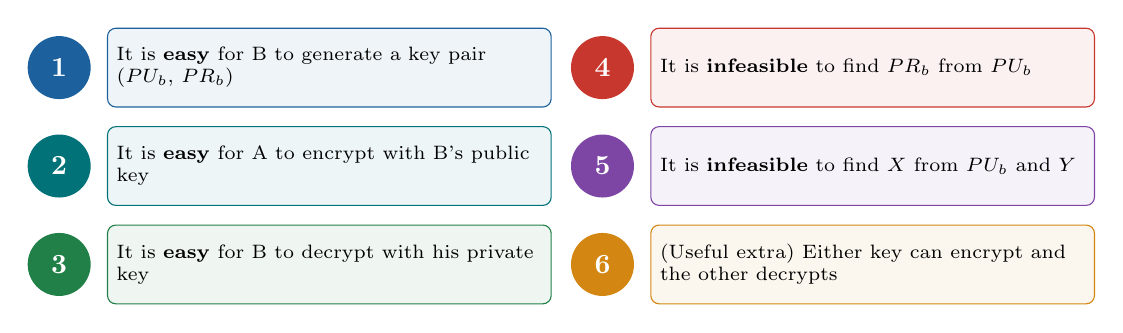
\begin{tikzpicture}
    \foreach \t/\c [count=\i] in {
      It is \textbf{easy} for B to generate a key pair ($PU_b$\comma{} $PR_b$)/ocean,
      It is \textbf{easy} for A to encrypt with B's public key/aqua!80!black,
      It is \textbf{easy} for B to decrypt with his private key/leaf!80!black,
      It is \textbf{infeasible} to find $PR_b$ from $PU_b$/brick,
      It is \textbf{infeasible} to find $X$ from $PU_b$ and $Y$/grape,
      (Useful extra) Either key can encrypt and the other decrypts/amber!90!black}
    {
      \pgfmathsetmacro{\x}{ifthenelse(\i<4,0,6.9)}
      \pgfmathsetmacro{\y}{-mod(\i-1,3)*1.25}
      \node[circle,fill=\c,text=white,font=\bfseries,minimum size=8mm] (c\i) at (\x,\y) {\i};
      \node[draw=\c,fill=\c!7,rounded corners=3pt,anchor=west,text width=54mm,minimum height=10mm,font=\scriptsize] at ([xshift=2mm]c\i.east) {\t};
    }
  \end{tikzpicture}
  \vspace{3mm}
  \begin{block}{Summed up}
    \small Easy for the \textbf{right person}, practically impossible for \textbf{everyone else}. These conditions were set out by Diffie and Hellman.
  \end{block}
\end{frame}

% ------------------------------------------------------------
\begin{frame}{The Trap-Door One-Way Function}
  \begin{columns}[c]
    \begin{column}{0.5\textwidth}
      \centering
      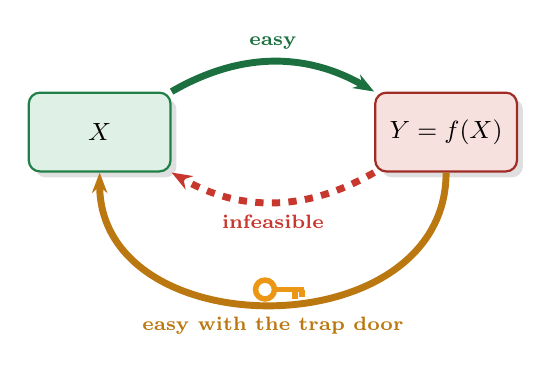
\begin{tikzpicture}
        \node[box=leaf,minimum width=18mm,minimum height=10mm] (x) at (0,0) {$X$};
        \node[box=brick,minimum width=18mm,minimum height=10mm] (y) at (4.4,0) {$Y = f(X)$};
        \draw[->,leaf!70!black,line width=2.5pt] (x.north east) to[bend left=30] node[above,font=\scriptsize\bfseries]{easy} (y.north west);
        \draw[->,brick,line width=2.5pt,dashed] (y.south west) to[bend left=30] node[below,font=\scriptsize\bfseries]{infeasible} (x.south east);
        \draw[->,amber!80!black,line width=2.5pt] (y.south) to[out=-90,in=-90,looseness=1.3] node[below,font=\scriptsize\bfseries]{easy \textbf{with the trap door}} (x.south);
        \pic at (2.1,-2.0) {key=amber};
      \end{tikzpicture}
    \end{column}
    \begin{column}{0.48\textwidth}
      \begin{block}{One-way function}
        \small Easy to compute in one direction, \textbf{infeasible to reverse}.
      \end{block}
      \begin{alertblock}{Trap-door one-way function}
        \small Infeasible to reverse \textbf{unless} you know a secret, the \textbf{trap door}. With it, reversing becomes easy.
      \end{alertblock}
      \begin{exampleblock}{Example}
        \small Multiplying two big primes is easy; \textbf{factoring} the product is hard. Knowing one factor is the trap door. This is the idea behind RSA.
      \end{exampleblock}
    \end{column}
  \end{columns}
\end{frame}

% ------------------------------------------------------------
\begin{frame}{Public-Key Cryptanalysis}
  \centering
  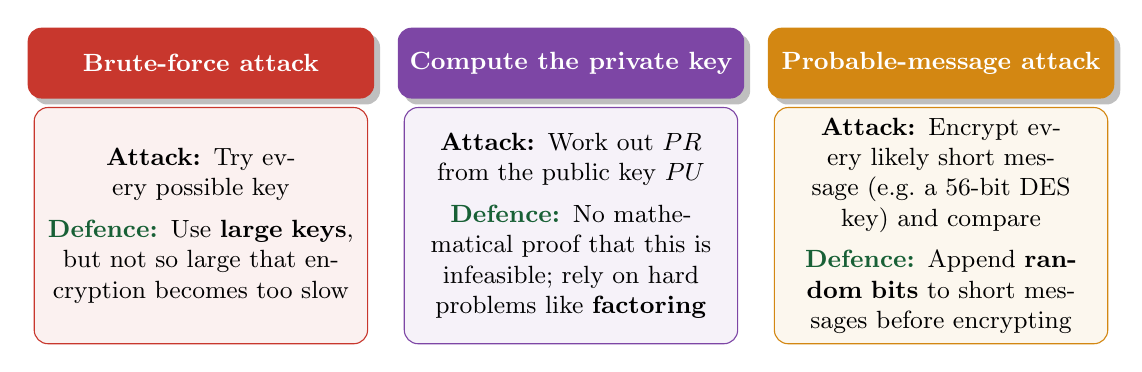
\begin{tikzpicture}
    \foreach \x/\c/\t/\d/\f in {
      0/brick/Brute-force attack/Try every possible key/Use \textbf{large keys}\comma{} but not so large that encryption becomes too slow,
      4.7/grape/Compute the private key/Work out $PR$ from the public key $PU$/No mathematical proof that this is infeasible; rely on hard problems like \textbf{factoring},
      9.4/amber!90!black/Probable-message attack/Encrypt every likely short message (e.g.\ a 56-bit DES key) and compare/Append \textbf{random bits} to short messages before encrypting}
    {
      \node[fill=\c,text=white,rounded corners=5pt,font=\small\bfseries,minimum width=44mm,minimum height=9mm,drop shadow] (h) at (\x,0) {\t};
      \node[draw=\c,fill=\c!7,rounded corners=5pt,text width=40mm,minimum height=30mm,font=\small,anchor=north,align=center] at ([yshift=-1mm]h.south) {\textbf{Attack:} \d\\[4pt]\textcolor{leaf!60!black}{\textbf{Defence:}} \f};
    }
  \end{tikzpicture}
\end{frame}

% ============================================================
\setcounter{section}{16}
\section{RSA and Diffie--Hellman Algorithms}
% ============================================================

\begin{frame}{The RSA Algorithm}
  \begin{columns}[c]
    \begin{column}{0.46\textwidth}
      \centering
      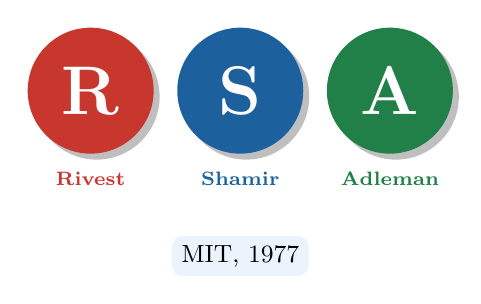
\begin{tikzpicture}
        \foreach \l/\n/\c [count=\i from 0] in {R/Rivest/brick,S/Shamir/ocean,A/Adleman/leaf!80!black}{
          \node[circle,fill=\c,text=white,font=\Huge\bfseries,minimum size=16mm,drop shadow] (c\i) at (\i*1.9,0) {\l};
          \node[font=\scriptsize\bfseries,text=\c,below=1mm of c\i] {\n};
        }
        \node[fill=sky,rounded corners,font=\small,align=center] at (1.9,-2.1) {MIT, 1977};
      \end{tikzpicture}
    \end{column}
    \begin{column}{0.52\textwidth}
      \begin{itemize}\small\setlength{\itemsep}{4pt}
        \item Named after its inventors, Rivest, Shamir and Adleman
        \item The most widely used public-key algorithm
        \item A \textbf{block cipher}: plaintext and ciphertext are integers between $0$ and $n-1$
        \item Can do all three jobs: encryption, signatures and key exchange
      \end{itemize}
      \begin{block}{Its security rests on}
        \small The difficulty of \textbf{factoring} a very large number $n$ into its two prime factors.
      \end{block}
    \end{column}
  \end{columns}
\end{frame}

% ------------------------------------------------------------
\begin{frame}{RSA Key Generation}
  \centering
  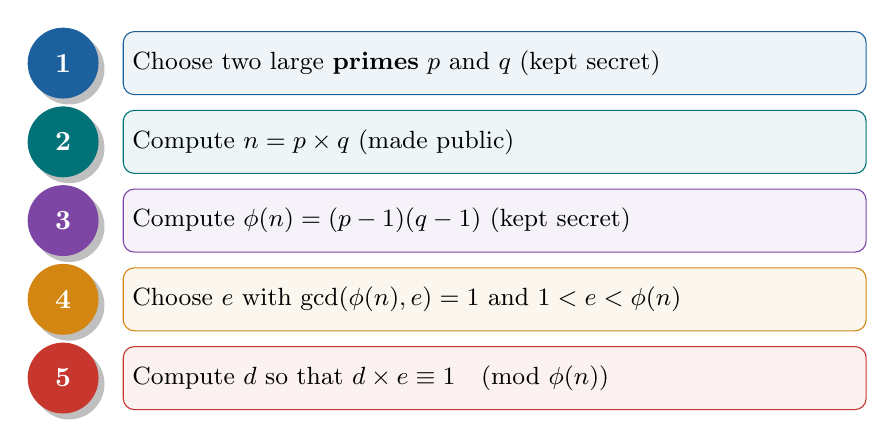
\begin{tikzpicture}
    \foreach \t/\c [count=\i] in {
      Choose two large \textbf{primes} $p$ and $q$ (kept secret)/ocean,
      Compute $n = p \times q$ (made public)/aqua!80!black,
      Compute $\phi(n) = (p-1)(q-1)$ (kept secret)/grape,
      Choose $e$ with $\gcd(\phi(n)\comma e) = 1$ and $1 < e < \phi(n)$/amber!90!black,
      Compute $d$ so that $d \times e \equiv 1 \pmod{\phi(n)}$/brick}
    {
      \node[circle,fill=\c,text=white,font=\bfseries,minimum size=9mm,drop shadow] (c\i) at (0,-\i*1.0) {\i};
      \node[draw=\c,fill=\c!7,rounded corners=4pt,anchor=west,text width=92mm,minimum height=8mm,font=\small] at ([xshift=3mm]c\i.east) {\t};
    }
  \end{tikzpicture}
  \vspace{3mm}
  \begin{columns}[T]
    \begin{column}{0.48\textwidth}
      \begin{exampleblock}{Public key}
        \centering $PU = \{e,\ n\}$
      \end{exampleblock}
    \end{column}
    \begin{column}{0.48\textwidth}
      \begin{alertblock}{Private key}
        \centering $PR = \{d,\ n\}$
      \end{alertblock}
    \end{column}
  \end{columns}
\end{frame}

% ------------------------------------------------------------
\begin{frame}{RSA Encryption and Decryption}
  \centering
  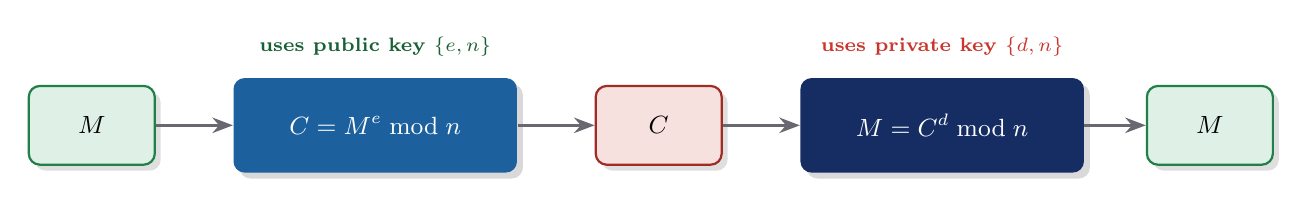
\begin{tikzpicture}
    \node[box=leaf,minimum width=16mm,minimum height=10mm] (m) at (0,0) {$M$};
    \node[solid box=ocean,minimum width=36mm,minimum height=12mm] (e) at (3.6,0) {$C = M^{e} \bmod n$};
    \node[box=brick,minimum width=16mm,minimum height=10mm] (c) at (7.2,0) {$C$};
    \node[solid box=navy,minimum width=36mm,minimum height=12mm] (d) at (10.8,0) {$M = C^{d} \bmod n$};
    \node[box=leaf,minimum width=16mm,minimum height=10mm] (m2) at (14.2,0) {$M$};
    \draw[flow] (m) -- (e); \draw[flow] (e) -- (c); \draw[flow] (c) -- (d); \draw[flow] (d) -- (m2);
    \node[font=\scriptsize\bfseries,text=leaf!60!black] at (3.6,1.0) {uses public key $\{e,n\}$};
    \node[font=\scriptsize\bfseries,text=brick] at (10.8,1.0) {uses private key $\{d,n\}$};
  \end{tikzpicture}
  \vspace{5mm}
  \begin{columns}[T]
    \begin{column}{0.48\textwidth}
      \begin{block}{Rules}
        \small The message $M$ must be \textbf{smaller than} $n$. A long message is split into blocks, each less than $n$.
      \end{block}
    \end{column}
    \begin{column}{0.48\textwidth}
      \begin{exampleblock}{Why it works}
        \small Because $ed \equiv 1 \pmod{\phi(n)}$, raising to the power $e$ and then $d$ gives back $M$: $\ (M^e)^d \bmod n = M$.
      \end{exampleblock}
    \end{column}
  \end{columns}
\end{frame}

% ------------------------------------------------------------
\begin{frame}{RSA Worked Example: Making the Keys}
  \begin{columns}[c]
    \begin{column}{0.56\textwidth}
      \centering
      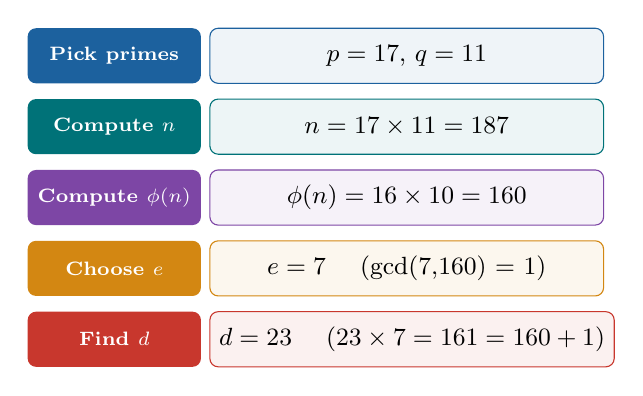
\begin{tikzpicture}
        \foreach \s/\v/\c [count=\i from 0] in {
          Pick primes/$p = 17$\comma\ $q = 11$/ocean,
          Compute $n$/$n = 17 \times 11 = 187$/aqua!80!black,
          Compute $\phi(n)$/$\phi(n) = 16 \times 10 = 160$/grape,
          Choose $e$/$e = 7$ \quad (gcd(7\comma 160) = 1)/amber!90!black,
          Find $d$/$d = 23$ \quad ($23 \times 7 = 161 = 160 + 1$)/brick}
        {
          \node[fill=\c,text=white,font=\scriptsize\bfseries,rounded corners=3pt,minimum width=22mm,minimum height=7mm] (h\i) at (0,-\i*0.9) {\s};
          \node[draw=\c,fill=\c!7,rounded corners=3pt,anchor=west,minimum width=50mm,minimum height=7mm,font=\small] at ([xshift=1mm]h\i.east) {\v};
        }
      \end{tikzpicture}
    \end{column}
    \begin{column}{0.42\textwidth}
      \begin{exampleblock}{Public key}
        \centering\Large $\{7,\ 187\}$
      \end{exampleblock}
      \begin{alertblock}{Private key}
        \centering\Large $\{23,\ 187\}$
      \end{alertblock}
      {\small Real RSA uses primes hundreds of digits long; small numbers just make the steps easy to follow.}
    \end{column}
  \end{columns}
\end{frame}

% ------------------------------------------------------------
\begin{frame}{RSA Worked Example: Encrypt and Decrypt}
  \centering
  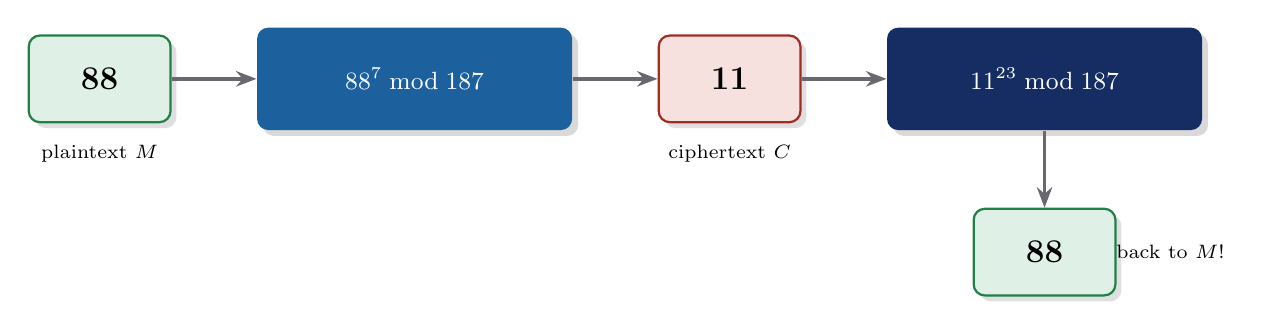
\begin{tikzpicture}
    \node[box=leaf,minimum width=18mm,minimum height=11mm,font=\large\bfseries] (m) at (0,0) {88};
    \node[solid box=ocean,minimum width=40mm,minimum height=13mm] (e) at (4.0,0) {$88^{7} \bmod 187$};
    \node[box=brick,minimum width=18mm,minimum height=11mm,font=\large\bfseries] (c) at (8.0,0) {11};
    \node[solid box=navy,minimum width=40mm,minimum height=13mm] (d) at (12.0,0) {$11^{23} \bmod 187$};
    \node[box=leaf,minimum width=18mm,minimum height=11mm,font=\large\bfseries] (m2) at (12.0,-2.2) {88};
    \draw[flow] (m) -- (e); \draw[flow] (e) -- (c); \draw[flow] (c) -- (d); \draw[flow] (d) -- (m2);
    \node[font=\scriptsize] at (0,-0.95) {plaintext $M$};
    \node[font=\scriptsize] at (8.0,-0.95) {ciphertext $C$};
    \node[font=\scriptsize] at (13.6,-2.2) {back to $M$!};
  \end{tikzpicture}
  \vspace{4mm}
  \begin{columns}[T]
    \begin{column}{0.48\textwidth}
      \begin{block}{Encryption (public key 7, 187)}
        \small $C = 88^{7} \bmod 187 = \mathbf{11}$
      \end{block}
    \end{column}
    \begin{column}{0.48\textwidth}
      \begin{alertblock}{Decryption (private key 23, 187)}
        \small $M = 11^{23} \bmod 187 = \mathbf{88}$
      \end{alertblock}
    \end{column}
  \end{columns}
\end{frame}

% ------------------------------------------------------------
\begin{frame}{Computational Aspects: Keeping Numbers Small}
  \begin{columns}[c]
    \begin{column}{0.5\textwidth}
      \begin{block}{The problem}
        \small $11^{23}$ is a 24-digit number; with real RSA keys, $C^{d}$ would have \textbf{billions of digits}. We cannot compute it directly.
      \end{block}
      \begin{exampleblock}{The trick: reduce as you go}
        \small $[(a \bmod n) \times (b \bmod n)] \bmod n = (a \times b) \bmod n$\\[3pt]
        So take ``mod $n$'' after \textbf{every} multiplication, and the numbers never grow bigger than $n^2$.
      \end{exampleblock}
    \end{column}
    \begin{column}{0.48\textwidth}
      \centering
      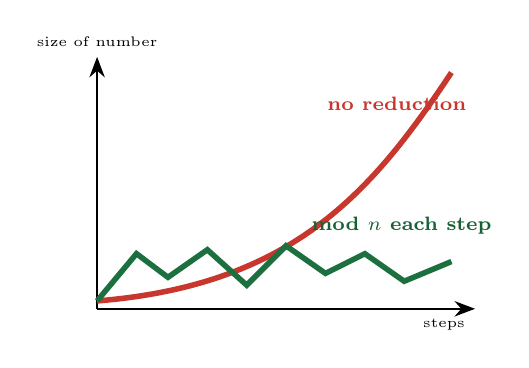
\begin{tikzpicture}
        \draw[->,thick] (0,0) -- (4.8,0) node[below left,font=\tiny]{steps};
        \draw[->,thick] (0,0) -- (0,3.2) node[above,font=\tiny]{size of number};
        \draw[brick,line width=2pt] (0,0.1) .. controls (2.5,0.3) and (3.5,1.5) .. (4.5,3.0);
        \node[font=\scriptsize\bfseries,text=brick,anchor=west] at (2.8,2.6) {no reduction};
        \draw[leaf!70!black,line width=2pt] (0,0.1) -- (0.5,0.7) -- (0.9,0.4) -- (1.4,0.75) -- (1.9,0.3) -- (2.4,0.8) -- (2.9,0.45) -- (3.4,0.7) -- (3.9,0.35) -- (4.5,0.6);
        \node[font=\scriptsize\bfseries,text=leaf!60!black,anchor=west] at (2.6,1.05) {mod $n$ each step};
      \end{tikzpicture}
    \end{column}
  \end{columns}
\end{frame}

% ------------------------------------------------------------
\begin{frame}{Fast Exponentiation: Square-and-Multiply}
  \begin{columns}[c]
    \begin{column}{0.55\textwidth}
      \centering
      {\small Compute $88^{7} \bmod 187$, with $7 = 4 + 2 + 1$:}\\[2mm]
      \renewcommand{\arraystretch}{1.35}
      \small
      \begin{tabular}{l l}
        \toprule
        \rowcolor{navy}\textcolor{white}{\textbf{Step}} & \textcolor{white}{\textbf{Value mod 187}}\\
        \midrule
        $88^{1}$ & 88\\
        $88^{2} = 7744$ & \textbf{77}\\
        $88^{4} = 77^2 = 5929$ & \textbf{132}\\
        \rowcolor{amber!15} $88^{7} = 88^{4}\cdot 88^{2}\cdot 88^{1}$ & $132 \times 77 \times 88 \bmod 187 = \mathbf{11}$\\
        \bottomrule
      \end{tabular}
    \end{column}
    \begin{column}{0.43\textwidth}
      \begin{itemize}\small\setlength{\itemsep}{4pt}
        \item Write the exponent in \textbf{binary} ($7 = 111_2$)
        \item Keep \textbf{squaring}: $x, x^2, x^4, x^8, \dots$
        \item \textbf{Multiply} together the powers whose bit is 1
        \item Reduce mod $n$ at every step
      \end{itemize}
      \begin{exampleblock}{Speed}
        \small A 1000-bit exponent needs about \textbf{2000} multiplications, not $2^{1000}$.
      \end{exampleblock}
    \end{column}
  \end{columns}
\end{frame}

% ------------------------------------------------------------
\begin{frame}{Efficient Operation Using the Public Key}
  \begin{columns}[c]
    \begin{column}{0.48\textwidth}
      \centering
      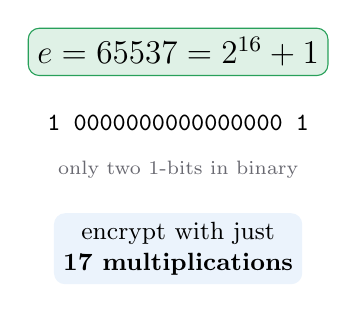
\begin{tikzpicture}
        \node[fill=leaf!15,draw=leaf,rounded corners,font=\large\bfseries] at (0,1.2) {$e = 65537 = 2^{16} + 1$};
        \node[font=\ttfamily\small] at (0,0.3) {1 0000000000000000 1};
        \node[font=\scriptsize,text=ink!70] at (0,-0.3) {only two 1-bits in binary};
        \node[fill=sky,rounded corners,font=\small,align=center] at (0,-1.3) {encrypt with just\\\textbf{17 multiplications}};
      \end{tikzpicture}
    \end{column}
    \begin{column}{0.5\textwidth}
      \begin{itemize}\small\setlength{\itemsep}{4pt}
        \item To speed up encryption, choose a \textbf{small, special} $e$
        \item Common choices: $e = 65537$, or $e = 3$ and $e = 17$
        \item Few 1-bits means few multiplications in square-and-multiply
        \item $e$ must still satisfy $\gcd(e, \phi(n)) = 1$
      \end{itemize}
      \begin{alertblock}{Caution with very small $e$}
        \small With $e = 3$, sending the \textbf{same message} to 3 people lets an attacker recover it. Add \textbf{random padding} to each message.
      \end{alertblock}
    \end{column}
  \end{columns}
\end{frame}

% ------------------------------------------------------------
\begin{frame}{Efficient Operation Using the Private Key: CRT}
  \begin{columns}[c]
    \begin{column}{0.52\textwidth}
      \centering
      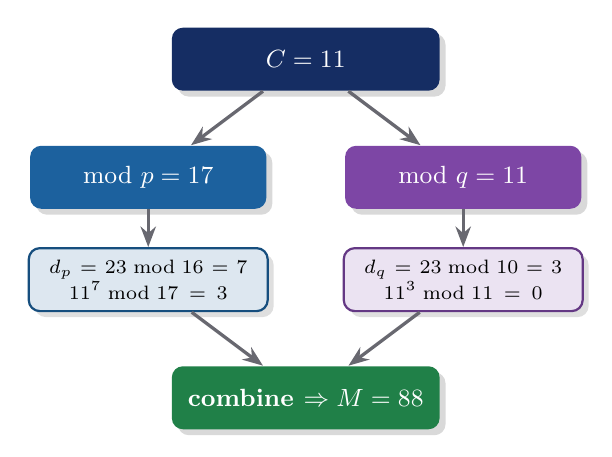
\begin{tikzpicture}
        \node[solid box=navy,minimum width=34mm] (c) at (0,0) {$C = 11$};
        \node[solid box=ocean,minimum width=30mm,font=\small] (p) at (-2.0,-1.5) {mod $p = 17$};
        \node[solid box=grape,minimum width=30mm,font=\small] (q) at (2.0,-1.5) {mod $q = 11$};
        \draw[flow] (c) -- (p); \draw[flow] (c) -- (q);
        \node[box=ocean,font=\scriptsize,text width=28mm,align=center] (mp) at (-2.0,-2.8) {$d_p = 23 \bmod 16 = 7$\\$11^{7} \bmod 17 = 3$};
        \node[box=grape,font=\scriptsize,text width=28mm,align=center] (mq) at (2.0,-2.8) {$d_q = 23 \bmod 10 = 3$\\$11^{3} \bmod 11 = 0$};
        \draw[flow] (p) -- (mp); \draw[flow] (q) -- (mq);
        \node[solid box=leaf!80!black,minimum width=34mm] (m) at (0,-4.3) {combine $\Rightarrow M = 88$};
        \draw[flow] (mp) -- (m); \draw[flow] (mq) -- (m);
      \end{tikzpicture}
    \end{column}
    \begin{column}{0.46\textwidth}
      \begin{block}{Chinese Remainder Theorem (CRT)}
        \small The owner of the private key knows $p$ and $q$. So instead of one big calculation mod $n$, do \textbf{two small} ones, mod $p$ and mod $q$, and combine them.
      \end{block}
      \begin{exampleblock}{Gain}
        \small Smaller numbers and smaller exponents: decryption becomes about \textbf{4 times faster}.
      \end{exampleblock}
      {\small Note: $d$ cannot be made small to save time; a small $d$ is easy to attack.}
    \end{column}
  \end{columns}
\end{frame}

% ------------------------------------------------------------
\begin{frame}{Generating the Keys in Practice}
  \centering
  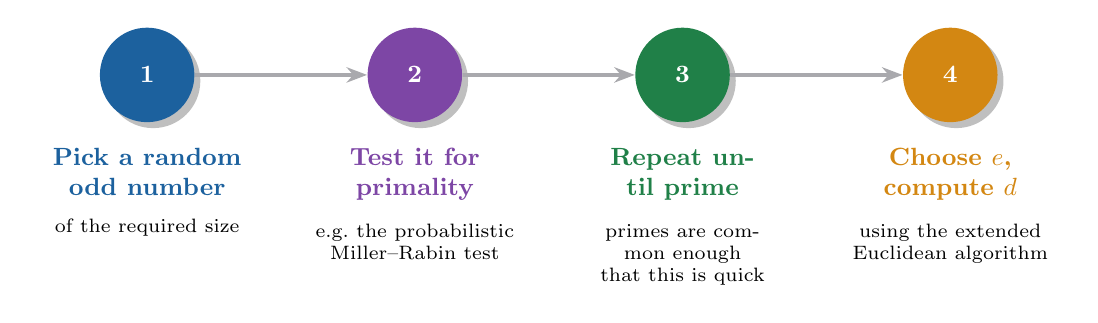
\begin{tikzpicture}
    \foreach \t/\d/\c [count=\i from 0] in {
      Pick a random odd number/of the required size/ocean,
      Test it for primality/e.g.\ the probabilistic Miller--Rabin test/grape,
      Repeat until prime/primes are common enough that this is quick/leaf!80!black,
      Choose $e$\comma{} compute $d$/using the extended Euclidean algorithm/amber!90!black}
    {
      \node[circle,fill=\c,text=white,font=\small\bfseries,minimum size=12mm,drop shadow] (s\i) at (\i*3.4,0) {\the\numexpr\i+1\relax};
      \node[font=\small\bfseries,text=\c,below=2mm of s\i,text width=28mm,align=center] (t\i) {\t};
      \node[font=\scriptsize,text width=28mm,align=center,below=0.5mm of t\i] {\d};
    }
    \foreach \i [evaluate=\i as \j using int(\i+1)] in {0,1,2} \draw[flow=ink!40] (s\i) -- (s\j);
  \end{tikzpicture}
  \vspace{4mm}
  \begin{alertblock}{Keep these secret}
    \small $p$, $q$ and $\phi(n)$ must never be revealed. Anyone who knows them can compute $d$ immediately.
  \end{alertblock}
\end{frame}

% ------------------------------------------------------------
\begin{frame}{The Security of RSA: Five Approaches to Attack}
  \centering
  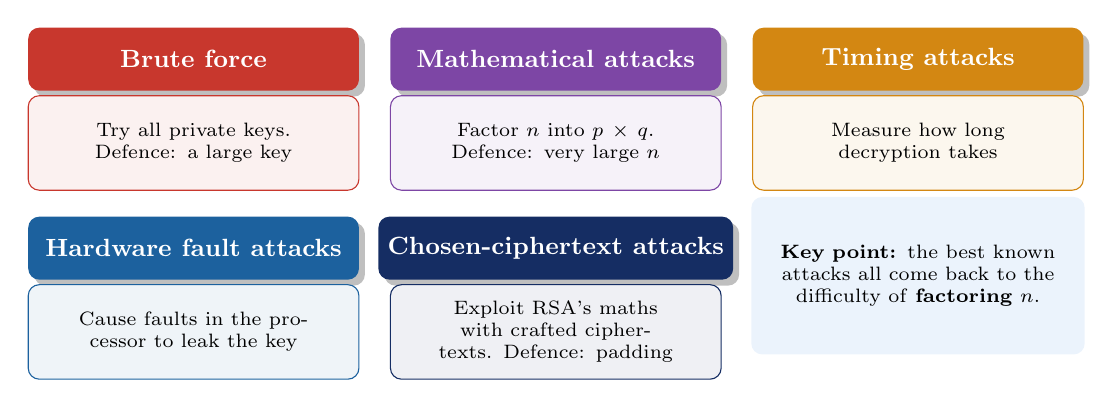
\begin{tikzpicture}
    \foreach \t/\d/\c [count=\i from 0] in {
      Brute force/Try all private keys. Defence: a large key/brick,
      Mathematical attacks/Factor $n$ into $p \times q$. Defence: very large $n$/grape,
      Timing attacks/Measure how long decryption takes/amber!90!black,
      Hardware fault attacks/Cause faults in the processor to leak the key/ocean,
      Chosen-ciphertext attacks/Exploit RSA's maths with crafted ciphertexts. Defence: padding/navy}
    {
      \pgfmathsetmacro{\x}{mod(\i,3)*4.6}
      \pgfmathsetmacro{\y}{-floor(\i/3)*2.4}
      \node[fill=\c,text=white,font=\small\bfseries,rounded corners=4pt,minimum width=42mm,minimum height=8mm,drop shadow] (h\i) at (\x,\y) {\t};
      \node[draw=\c,fill=\c!7,rounded corners=4pt,minimum width=42mm,minimum height=12mm,text width=39mm,align=center,font=\scriptsize,anchor=north] at ([yshift=-0.5mm]h\i.south) {\d};
    }
    \node[fill=sky,rounded corners,text width=40mm,align=center,font=\scriptsize,minimum height=20mm] at (9.2,-2.75) {\textbf{Key point:} the best known attacks all come back to the difficulty of \textbf{factoring} $n$.};
  \end{tikzpicture}
\end{frame}

% ------------------------------------------------------------
\begin{frame}{The Factoring Problem and Key Size}
  \begin{columns}[c]
    \begin{column}{0.5\textwidth}
      \centering
      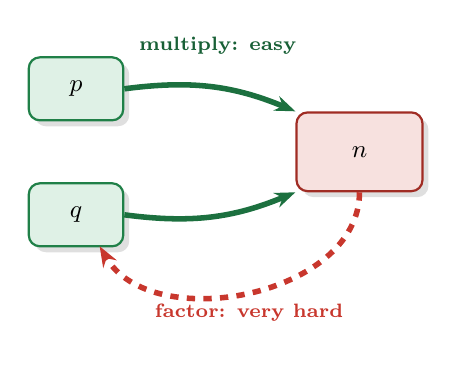
\begin{tikzpicture}
        \node[box=leaf,minimum width=12mm] (p) at (0,0.8) {$p$};
        \node[box=leaf,minimum width=12mm] (q) at (0,-0.8) {$q$};
        \node[box=brick,minimum width=16mm,minimum height=10mm] (n) at (3.6,0) {$n$};
        \draw[->,leaf!70!black,line width=2pt] (p.east) to[bend left=15] (n.north west);
        \draw[->,leaf!70!black,line width=2pt] (q.east) to[bend right=15] (n.south west);
        \node[font=\scriptsize\bfseries,text=leaf!60!black] at (1.8,1.35) {multiply: easy};
        \draw[->,brick,line width=2pt,dashed] (n.south) to[out=-90,in=-60] node[below,font=\scriptsize\bfseries,text=brick]{factor: very hard} (0.3,-1.2);
      \end{tikzpicture}
    \end{column}
    \begin{column}{0.48\textwidth}
      \begin{itemize}\small\setlength{\itemsep}{4pt}
        \item Multiplying $p \times q$ takes a moment
        \item Finding $p$ and $q$ from a huge $n$ is believed to be \textbf{infeasible}
        \item Factoring methods and computers keep improving, so key sizes keep \textbf{growing}
      \end{itemize}
      \begin{block}{Key sizes}
        \small Small keys (a few hundred bits) have been factored. Today \textbf{2048 bits} or more is recommended.
      \end{block}
    \end{column}
  \end{columns}
\end{frame}

% ------------------------------------------------------------
\begin{frame}{Timing Attacks on RSA and Countermeasures}
  \begin{columns}[c]
    \begin{column}{0.46\textwidth}
      \begin{alertblock}{The attack}
        \small Square-and-multiply does an \textbf{extra multiplication} for every 1-bit of $d$. By timing many decryptions, an attacker can work out the bits of $d$, one by one.
      \end{alertblock}
      {\small Like a burglar learning a safe's combination by listening to the clicks.}
    \end{column}
    \begin{column}{0.52\textwidth}
      \centering
      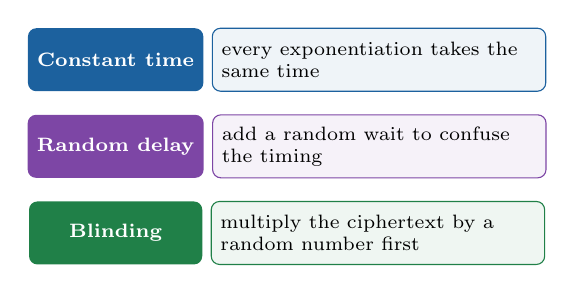
\begin{tikzpicture}
        \foreach \t/\d/\c [count=\i from 0] in {Constant time/every exponentiation takes the same time/ocean,Random delay/add a random wait to confuse the timing/grape,Blinding/multiply the ciphertext by a random number first/leaf!80!black}{
          \node[fill=\c,text=white,font=\scriptsize\bfseries,rounded corners=3pt,minimum width=22mm,minimum height=8mm] (h\i) at (0,-\i*1.1) {\t};
          \node[draw=\c,fill=\c!7,rounded corners=3pt,anchor=west,text width=40mm,minimum height=8mm,font=\scriptsize] at ([xshift=1mm]h\i.east) {\d};
        }
      \end{tikzpicture}
    \end{column}
  \end{columns}
\end{frame}

% ------------------------------------------------------------
\begin{frame}{Diffie--Hellman Key Exchange}
  \begin{columns}[c]
    \begin{column}{0.48\textwidth}
      \centering
      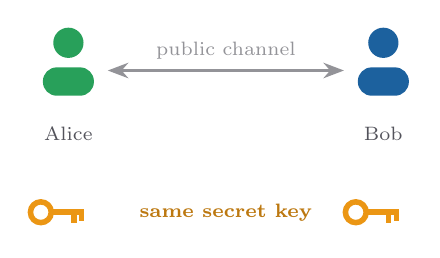
\begin{tikzpicture}
        \pic[scale=1.2] at (0,0) {person=leaf}; \node[tag] at (0,-0.6) {Alice};
        \pic[scale=1.2] at (4,0) {person=ocean}; \node[tag] at (4,-0.6) {Bob};
        \draw[<->,very thick,ink!50] (0.5,0.2) -- node[above,font=\scriptsize]{public channel} (3.5,0.2);
        \pic[scale=1.1] at (-0.35,-1.6) {key=amber}; \pic[scale=1.1] at (3.65,-1.6) {key=amber};
        \node[font=\scriptsize\bfseries,text=amber!80!black] at (2,-1.6) {same secret key};
      \end{tikzpicture}
    \end{column}
    \begin{column}{0.5\textwidth}
      \begin{itemize}\small\setlength{\itemsep}{4pt}
        \item Published by \textbf{Diffie and Hellman in 1976}: the first public-key algorithm
        \item Purpose: let two users \textbf{agree on a secret key} over a public channel
        \item It does \textbf{not} encrypt messages; the agreed key is then used with a symmetric cipher
      \end{itemize}
      \begin{block}{Security based on}
        \small The difficulty of computing \textbf{discrete logarithms}.
      \end{block}
    \end{column}
  \end{columns}
\end{frame}

% ------------------------------------------------------------
\begin{frame}{Primitive Roots and Discrete Logarithms}
  \begin{columns}[c]
    \begin{column}{0.48\textwidth}
      \centering
      {\small Powers of 3 modulo 7:}\\[2mm]
      \renewcommand{\arraystretch}{1.3}
      \begin{tabular}{c|cccccc}
        \rowcolor{navy}\textcolor{white}{$i$} & \textcolor{white}{1} & \textcolor{white}{2} & \textcolor{white}{3} & \textcolor{white}{4} & \textcolor{white}{5} & \textcolor{white}{6}\\
        $3^{i} \bmod 7$ & 3 & 2 & 6 & 4 & 5 & 1\\
      \end{tabular}\\[3mm]
      {\small Every value 1--6 appears exactly once,\\so 3 is a \textbf{primitive root} of 7.}
    \end{column}
    \begin{column}{0.5\textwidth}
      \begin{block}{Primitive root}
        \small $\alpha$ is a primitive root of prime $q$ if its powers produce \textbf{all} the numbers $1$ to $q-1$.
      \end{block}
      \begin{alertblock}{Discrete logarithm}
        \small Given $y = \alpha^{x} \bmod q$, find $x$. Computing $y$ from $x$ is \textbf{easy}; finding $x$ from $y$ is \textbf{very hard} for large $q$.
      \end{alertblock}
      {\small Example: $3^{x} \bmod 7 = 4$ gives $x = 4$. Easy here, impossible when $q$ has hundreds of digits.}
    \end{column}
  \end{columns}
\end{frame}

% ------------------------------------------------------------
\begin{frame}{The Diffie--Hellman Algorithm}
  \centering
  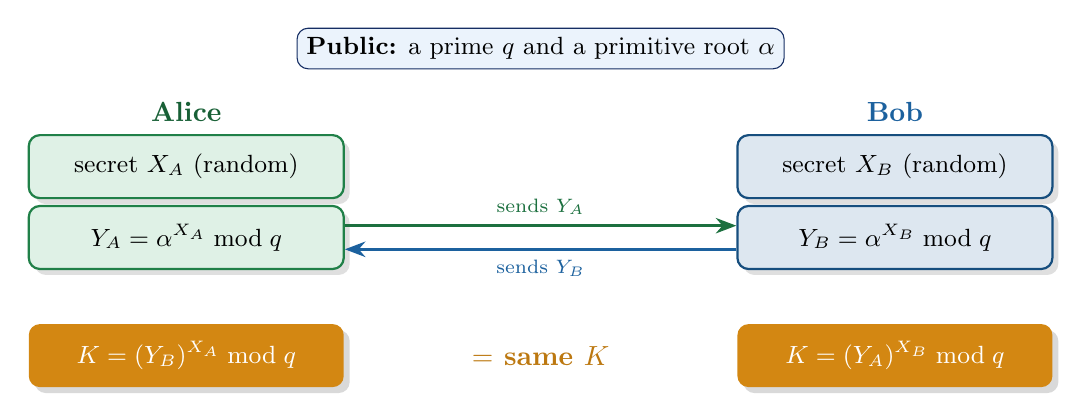
\begin{tikzpicture}
    \node[fill=sky,draw=navy,rounded corners,font=\small,minimum width=60mm] at (4.5,1.5) {\textbf{Public:} a prime $q$ and a primitive root $\alpha$};
    \node[font=\bfseries,text=leaf!60!black] at (0,0.7) {Alice};
    \node[font=\bfseries,text=ocean] at (9,0.7) {Bob};
    \node[box=leaf,minimum width=40mm,font=\small] (a1) at (0,0) {secret $X_A$ (random)};
    \node[box=leaf,minimum width=40mm,font=\small] (a2) at (0,-0.9) {$Y_A = \alpha^{X_A} \bmod q$};
    \node[box=ocean,minimum width=40mm,font=\small] (b1) at (9,0) {secret $X_B$ (random)};
    \node[box=ocean,minimum width=40mm,font=\small] (b2) at (9,-0.9) {$Y_B = \alpha^{X_B} \bmod q$};
    \draw[->,very thick,leaf!70!black] ([yshift=1.5mm]a2.east) -- node[above,font=\scriptsize]{sends $Y_A$} ([yshift=1.5mm]b2.west);
    \draw[->,very thick,ocean] ([yshift=-1.5mm]b2.west) -- node[below,font=\scriptsize]{sends $Y_B$} ([yshift=-1.5mm]a2.east);
    \node[solid box=amber!90!black,minimum width=40mm,font=\small] (a3) at (0,-2.4) {$K = (Y_B)^{X_A} \bmod q$};
    \node[solid box=amber!90!black,minimum width=40mm,font=\small] (b3) at (9,-2.4) {$K = (Y_A)^{X_B} \bmod q$};
    \node[font=\bfseries,text=amber!80!black] at (4.5,-2.4) {$=$ same $K$};
  \end{tikzpicture}
  \vspace{2mm}

  {\small An eavesdropper sees $q$, $\alpha$, $Y_A$ and $Y_B$, but finding $K$ needs a \textbf{discrete logarithm}.}
\end{frame}

% ------------------------------------------------------------
\begin{frame}{Diffie--Hellman Worked Example}
  \centering
  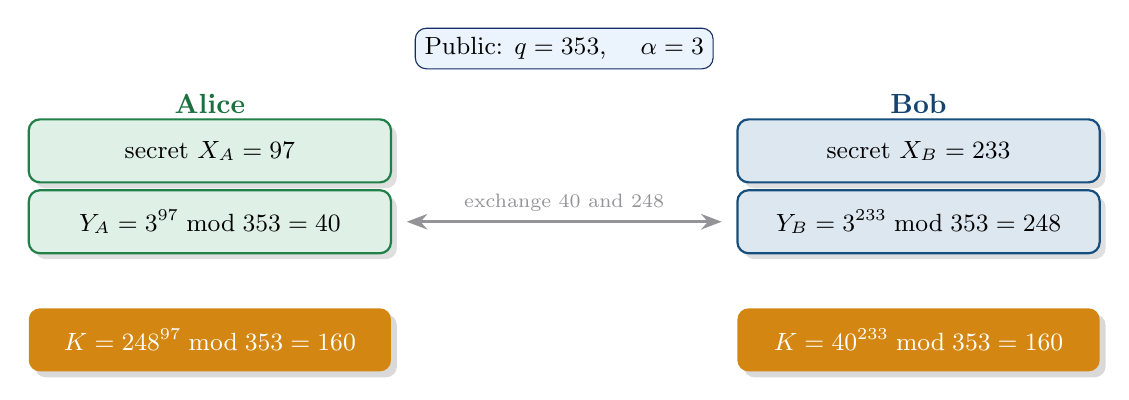
\begin{tikzpicture}
    \node[fill=sky,draw=navy,rounded corners,font=\small] at (4.5,1.3) {Public: $q = 353$, \quad $\alpha = 3$};
    \foreach \l/\x/\c/\s/\y/\k in {Alice/0/leaf/X_A = 97/Y_A = 3^{97} \bmod 353 = 40/K = 248^{97} \bmod 353 = 160,Bob/9/ocean/X_B = 233/Y_B = 3^{233} \bmod 353 = 248/K = 40^{233} \bmod 353 = 160}{
      \node[font=\bfseries,text=\c!70!black] at (\x,0.6) {\l};
      \node[box=\c,minimum width=46mm,font=\small] at (\x,0) {secret $\s$};
      \node[box=\c,minimum width=46mm,font=\small] at (\x,-0.9) {$\y$};
      \node[solid box=amber!90!black,minimum width=46mm,font=\small] at (\x,-2.4) {$\k$};
    }
    \draw[<->,very thick,ink!50] (2.5,-0.9) -- node[above,font=\scriptsize]{exchange 40 and 248} (6.5,-0.9);
  \end{tikzpicture}
  \vspace{3mm}
  \begin{block}{Result}
    \small Both compute the shared secret \textbf{$K = 160$}. An attacker sees only 353, 3, 40 and 248. Here 97 could be found by trial, but with large numbers it is impossible.
  \end{block}
\end{frame}

% ------------------------------------------------------------
\begin{frame}{An Analogy: Mixing Paint}
  \centering
  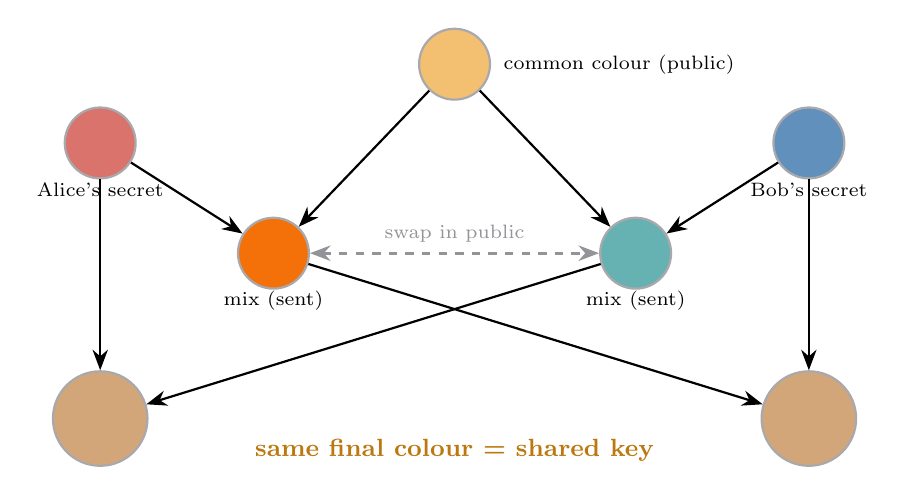
\begin{tikzpicture}[blob/.style={circle,minimum size=9mm,draw=ink!40,thick}]
    \node[blob,fill=amber!60] (c) at (4.5,1.6) {};
    \node[font=\scriptsize,anchor=west] at (5.0,1.6) {common colour (public)};
    \node[blob,fill=brick!70] (as) at (0,0.6) {}; \node[font=\scriptsize] at (0,0.0) {Alice's secret};
    \node[blob,fill=ocean!70] (bs) at (9,0.6) {}; \node[font=\scriptsize] at (9,0.0) {Bob's secret};
    \node[blob,fill=orange!80!brick] (am) at (2.2,-0.8) {}; \node[font=\scriptsize] at (2.2,-1.4) {mix (sent)};
    \node[blob,fill=teal!60] (bm) at (6.8,-0.8) {}; \node[font=\scriptsize] at (6.8,-1.4) {mix (sent)};
    \draw[->,thick] (c) -- (am); \draw[->,thick] (as) -- (am); \draw[->,thick] (c) -- (bm); \draw[->,thick] (bs) -- (bm);
    \draw[<->,very thick,ink!50,dashed] (am) -- node[above,font=\scriptsize]{swap in public} (bm);
    \node[blob,fill=brown!70,minimum size=12mm] (k1) at (0,-2.9) {}; \node[blob,fill=brown!70,minimum size=12mm] (k2) at (9,-2.9) {};
    \draw[->,thick] (bm) -- (k1); \draw[->,thick] (as) -- (k1);
    \draw[->,thick] (am) -- (k2); \draw[->,thick] (bs) -- (k2);
    \node[font=\small\bfseries,text=amber!80!black] at (4.5,-3.3) {same final colour = shared key};
  \end{tikzpicture}\par
  {\small Mixing paint is easy; \textbf{un-mixing} it to find someone's secret colour is practically impossible. That is exactly the role of the discrete logarithm.}
\end{frame}

% ------------------------------------------------------------
\begin{frame}{The Man-in-the-Middle Attack}
  \centering
  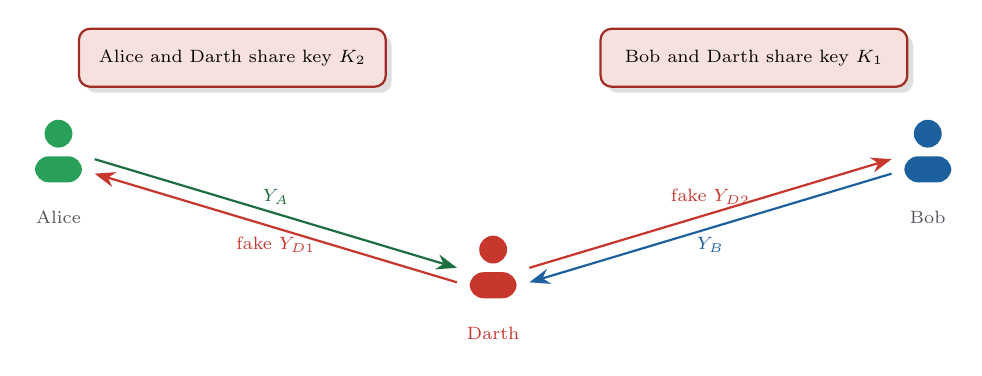
\begin{tikzpicture}[scale=0.92,transform shape]
    \pic[scale=1.2] at (0,0) {person=leaf}; \node[tag] at (0,-0.6) {Alice};
    \pic[scale=1.2] at (6,-1.6) {person=brick}; \node[tag,text=brick] at (6,-2.2) {Darth};
    \pic[scale=1.2] at (12,0) {person=ocean}; \node[tag] at (12,-0.6) {Bob};
    \draw[->,thick,leaf!70!black] (0.5,0.2) -- node[above,font=\scriptsize]{$Y_A$} (5.5,-1.3);
    \draw[->,thick,brick] (6.5,-1.3) -- node[above,font=\scriptsize]{fake $Y_{D2}$} (11.5,0.2);
    \draw[->,thick,ocean] (11.5,0.0) -- node[below,font=\scriptsize]{$Y_B$} (6.5,-1.5);
    \draw[->,thick,brick] (5.5,-1.5) -- node[below,font=\scriptsize]{fake $Y_{D1}$} (0.5,0.0);
    \node[box=brick,font=\scriptsize,text width=40mm,align=center] at (2.4,1.6) {Alice and Darth share key $K_2$};
    \node[box=brick,font=\scriptsize,text width=40mm,align=center] at (9.6,1.6) {Bob and Darth share key $K_1$};
  \end{tikzpicture}
  \vspace{1mm}
  \begin{columns}[T]
    \begin{column}{0.48\textwidth}
      \begin{alertblock}{What goes wrong}
        \small Darth intercepts both public values and sends his \textbf{own} instead. Alice and Bob each think they share a key with the other, but both share keys with \textbf{Darth}.
      \end{alertblock}
    \end{column}
    \begin{column}{0.48\textwidth}
      \begin{block}{Result}
        \small Darth decrypts every message, reads or changes it, re-encrypts it and passes it on. Nobody notices.
      \end{block}
    \end{column}
  \end{columns}
\end{frame}

% ------------------------------------------------------------
\begin{frame}{Why MITM Works, and How to Stop It}
  \begin{columns}[c]
    \begin{column}{0.48\textwidth}
      \begin{alertblock}{The root cause}
        \small Basic Diffie--Hellman does \textbf{not authenticate} the participants. Alice cannot tell whether $Y_B$ really came from Bob.
      \end{alertblock}
      \centering
      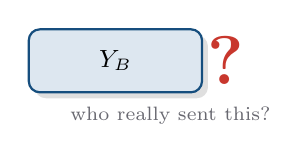
\begin{tikzpicture}
        \node[box=ocean,font=\small] (y) at (0,0) {$Y_B$};
        \node[font=\Huge\bfseries,text=brick] at (1.4,0) {?};
        \node[font=\scriptsize,text=ink!70] at (0.7,-0.7) {who really sent this?};
      \end{tikzpicture}
    \end{column}
    \begin{column}{0.5\textwidth}
      \centering
      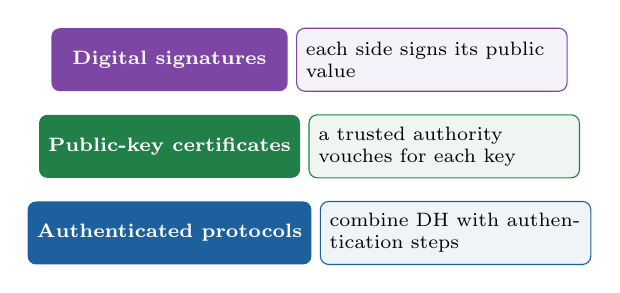
\begin{tikzpicture}
        \foreach \t/\d/\c [count=\i from 0] in {Digital signatures/each side signs its public value/grape,Public-key certificates/a trusted authority vouches for each key/leaf!80!black,Authenticated protocols/combine DH with authentication steps/ocean}{
          \node[fill=\c,text=white,font=\scriptsize\bfseries,rounded corners=3pt,minimum width=30mm,minimum height=8mm] (h\i) at (0,-\i*1.1) {\t};
          \node[draw=\c,fill=\c!7,rounded corners=3pt,anchor=west,text width=32mm,minimum height=8mm,font=\scriptsize] at ([xshift=1mm]h\i.east) {\d};
        }
      \end{tikzpicture}\\[2mm]
      {\small This is why we need \textbf{authentication} and \textbf{PKI}, studied in Modules 10--11.}
    \end{column}
  \end{columns}
\end{frame}

% ------------------------------------------------------------
\begin{frame}{RSA vs.\ Diffie--Hellman}
  \centering
  \renewcommand{\arraystretch}{1.45}
  \small
  \begin{tabular}{>{\bfseries}l >{\columncolor{brick!8}}c >{\columncolor{amber!10}}c}
    \toprule
    \rowcolor{navy}\textcolor{white}{Feature} & \textcolor{white}{\textbf{RSA}} & \textcolor{white}{\textbf{Diffie--Hellman}}\\
    \midrule
    Year & 1977 & 1976\\
    Hard problem & Factoring $n = pq$ & Discrete logarithm mod $q$\\
    Encryption & Yes & No\\
    Digital signature & Yes & No\\
    Key exchange & Yes & Yes (its only purpose)\\
    Main weakness & Slow; needs large keys & No authentication (MITM)\\
    \bottomrule
  \end{tabular}
\end{frame}

% ============================================================
\setcounter{section}{18}
\section{Elliptic Curve Cryptography}
% ============================================================

\begin{frame}{Why Elliptic Curve Cryptography?}
  \begin{columns}[c]
    \begin{column}{0.54\textwidth}
      \centering
      {\small Key sizes (bits) for \textbf{equal security}}\\[2mm]
      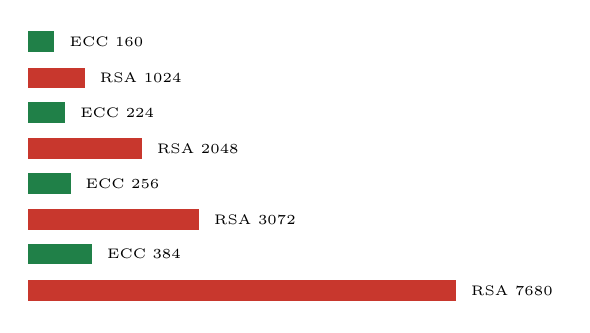
\begin{tikzpicture}[x=0.85mm]
        \foreach \ecc/\rsa/\y in {160/1024/0,224/2048/-0.9,256/3072/-1.8,384/7680/-2.7}{
          \fill[leaf!80!black] (0,\y+0.12) rectangle (\ecc/40,\y+0.38);
          \node[font=\tiny,anchor=west] at (\ecc/40+0.8,\y+0.25) {ECC \ecc};
          \fill[brick] (0,\y-0.34) rectangle (\rsa/120,\y-0.08);
          \node[font=\tiny,anchor=west] at (\rsa/120+0.8,\y-0.21) {RSA \rsa};
        }
      \end{tikzpicture}
    \end{column}
    \begin{column}{0.44\textwidth}
      \begin{itemize}\small\setlength{\itemsep}{4pt}
        \item RSA keys have had to grow very large, which makes RSA \textbf{slow}
        \item ECC gives the \textbf{same security} with much \textbf{smaller keys}
        \item Smaller keys mean less computing, less memory and less battery
      \end{itemize}
      \begin{exampleblock}{Where it shines}
        \small Smart cards, mobile phones and other small devices.
      \end{exampleblock}
    \end{column}
  \end{columns}
\end{frame}

% ------------------------------------------------------------
\begin{frame}{What Is an Elliptic Curve?}
  \begin{columns}[c]
    \begin{column}{0.5\textwidth}
      \centering
      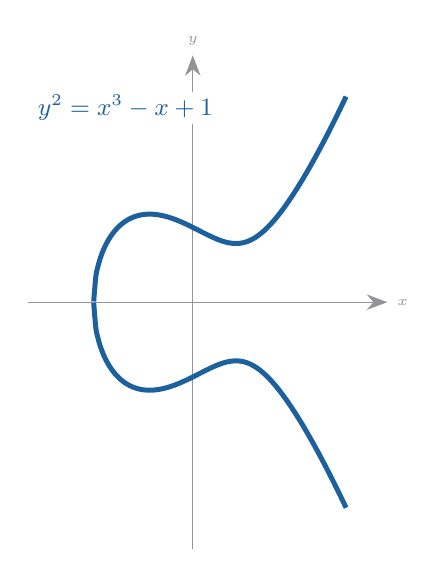
\begin{tikzpicture}[scale=0.95]
        \draw[->,ink!50] (-2.2,0) -- (2.6,0) node[right,font=\tiny]{$x$};
        \draw[->,ink!50] (0,-3.3) -- (0,3.3) node[above,font=\tiny]{$y$};
        \draw[ocean,line width=1.8pt,smooth,samples=120,domain=-1.3247:2.05] plot (\x,{sqrt(max(0,\x*\x*\x-\x+1))});
        \draw[ocean,line width=1.8pt,smooth,samples=120,domain=-1.3247:2.05] plot (\x,{-sqrt(max(0,\x*\x*\x-\x+1))});
        \node[font=\small,text=ocean,fill=white,inner sep=1pt] at (-0.9,2.6) {$y^2 = x^3 - x + 1$};
      \end{tikzpicture}
    \end{column}
    \begin{column}{0.48\textwidth}
      \begin{block}{Equation}
        \centering $y^{2} = x^{3} + ax + b$
      \end{block}
      \begin{itemize}\small\setlength{\itemsep}{3pt}
        \item The set of points $(x, y)$ that satisfy the equation
        \item Plus one extra point, the \textbf{point at infinity} $O$, which acts like zero
        \item The curve is \textbf{symmetric} about the $x$-axis
        \item Not an ellipse! The name comes from formulas for an ellipse's perimeter
      \end{itemize}
      {\small Condition: $4a^3 + 27b^2 \neq 0$, so the curve has no sharp points.}
    \end{column}
  \end{columns}
\end{frame}

% ------------------------------------------------------------
\begin{frame}{Adding Two Points: The Geometric Rule}
  \begin{columns}[c]
    \begin{column}{0.5\textwidth}
      \centering
      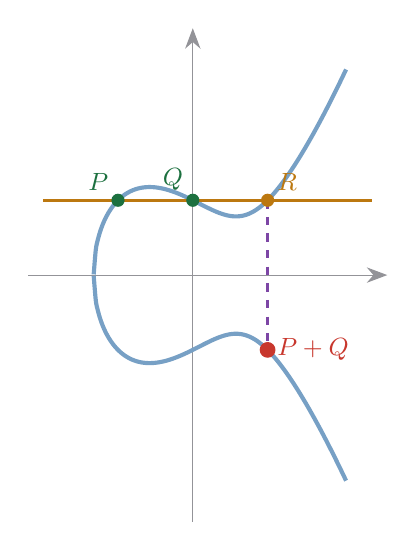
\begin{tikzpicture}[scale=0.95]
        \draw[->,ink!50] (-2.2,0) -- (2.6,0);
        \draw[->,ink!50] (0,-3.3) -- (0,3.3);
        \draw[ocean!60,line width=1.5pt,smooth,samples=120,domain=-1.3247:2.05] plot (\x,{sqrt(max(0,\x*\x*\x-\x+1))});
        \draw[ocean!60,line width=1.5pt,smooth,samples=120,domain=-1.3247:2.05] plot (\x,{-sqrt(max(0,\x*\x*\x-\x+1))});
        \draw[amber!80!black,very thick] (-2.0,1) -- (2.4,1);
        \draw[grape,very thick,dashed] (1,1) -- (1,-1);
        \fill[leaf!70!black] (-1,1) circle (2.5pt) node[above left,font=\small\bfseries] {$P$};
        \fill[leaf!70!black] (0,1) circle (2.5pt) node[above left,font=\small\bfseries] {$Q$};
        \fill[amber!80!black] (1,1) circle (2.5pt) node[above right,font=\small\bfseries] {$R$};
        \fill[brick] (1,-1) circle (3pt) node[right,font=\small\bfseries,text=brick] {$P + Q$};
      \end{tikzpicture}
    \end{column}
    \begin{column}{0.48\textwidth}
      \begin{enumerate}\small\setlength{\itemsep}{4pt}
        \item Draw the \textbf{line} through $P$ and $Q$
        \item It meets the curve at a \textbf{third point} $R$
        \item \textbf{Reflect} $R$ in the $x$-axis
        \item The result is $P + Q$
      \end{enumerate}
      \begin{exampleblock}{On this curve}
        \small $P = (-1, 1)$, $Q = (0, 1)$: the line $y = 1$ meets the curve again at $(1, 1)$, so $P + Q = (1, -1)$.
      \end{exampleblock}
      {\small \textbf{Doubling}: to get $P + P = 2P$, use the \textbf{tangent} line at $P$.}
    \end{column}
  \end{columns}
\end{frame}

% ------------------------------------------------------------
\begin{frame}{Elliptic Curves over a Finite Field}
  \begin{columns}[c]
    \begin{column}{0.52\textwidth}
      \centering
      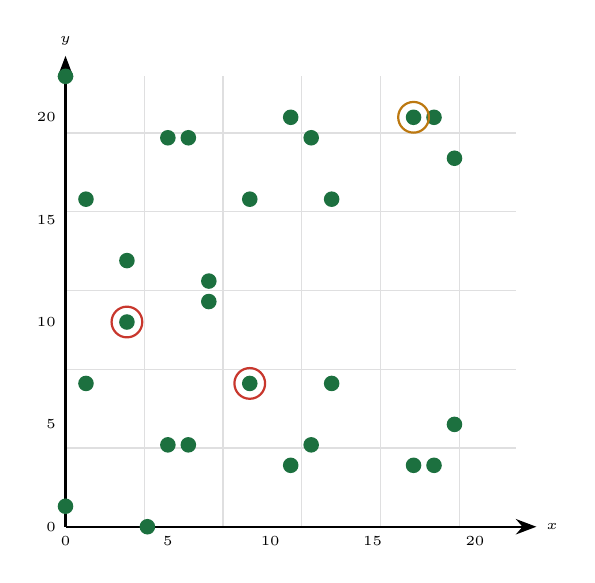
\begin{tikzpicture}[x=2.6mm,y=2.6mm]
        \draw[ink!15] (0,0) grid (22,22);
        \draw[->,thick] (0,0) -- (23,0) node[right,font=\tiny]{$x$};
        \draw[->,thick] (0,0) -- (0,23) node[above,font=\tiny]{$y$};
        \foreach \v in {0,5,10,15,20} {\node[font=\tiny,anchor=north] at (\v,0) {\v}; \node[font=\tiny,anchor=east] at (0,\v) {\v};}
        \foreach \p in {(0,1),(0,22),(1,7),(1,16),(3,10),(3,13),(4,0),(5,4),(5,19),(6,4),(6,19),(7,11),(7,12),(9,7),(9,16),(11,3),(11,20),(12,4),(12,19),(13,7),(13,16),(17,3),(17,20),(18,3),(18,20),(19,5),(19,18)}
          \fill[leaf!70!black] \p circle (0.38);
        \draw[brick,thick] (3,10) circle (0.75); \draw[brick,thick] (9,7) circle (0.75);
        \draw[amber!80!black,thick] (17,20) circle (0.75);
      \end{tikzpicture}
    \end{column}
    \begin{column}{0.46\textwidth}
      \begin{itemize}\small\setlength{\itemsep}{3pt}
        \item Cryptography uses whole numbers, so we work \textbf{modulo a prime} $p$
        \item $E_p(a, b)$: all $(x, y)$ with $y^2 \equiv x^3 + ax + b \pmod p$
        \item The chart shows $E_{23}(1, 1)$: \textbf{27 points} plus $O$
        \item The ``curve'' becomes a scatter of dots, but the same addition rules work
      \end{itemize}
      \begin{block}{Check a point}
        \small $(3, 10)$: $10^2 = 100 \equiv 8$ and $3^3 + 3 + 1 = 31 \equiv 8 \pmod{23}$ \good{\checkmark}
      \end{block}
    \end{column}
  \end{columns}
\end{frame}

% ------------------------------------------------------------
\begin{frame}{Point Addition Formulas: Worked Example}
  \begin{columns}[T]
    \begin{column}{0.48\textwidth}
      \begin{block}{Formulas for $P + Q = (x_R, y_R)$}
        \small
        $\lambda = \dfrac{y_Q - y_P}{x_Q - x_P}$ \quad (if $P \neq Q$)\\[4pt]
        $\lambda = \dfrac{3x_P^2 + a}{2y_P}$ \quad (if $P = Q$)\\[4pt]
        $x_R = \lambda^2 - x_P - x_Q$\\[2pt]
        $y_R = \lambda(x_P - x_R) - y_P$\\[2pt]
        all calculations mod $p$; ``division'' means multiplying by the inverse
      \end{block}
    \end{column}
    \begin{column}{0.5\textwidth}
      \begin{exampleblock}{In $E_{23}(1,1)$: $P = (3,10)$, $Q = (9,7)$}
        \small
        $\lambda = (7-10)/(9-3) = -3/6 \equiv 11$\\
        $x_R = 121 - 3 - 9 = 109 \equiv 17$\\
        $y_R = 11(3 - 17) - 10 = -164 \equiv 20$\\[3pt]
        $\Rightarrow\ P + Q = \mathbf{(17, 20)}$
      \end{exampleblock}
      \begin{exampleblock}{Doubling: $2P$}
        \small $\lambda = (27 + 1)/20 \equiv 6$, giving $2P = \mathbf{(7, 12)}$
      \end{exampleblock}
    \end{column}
  \end{columns}
\end{frame}

% ------------------------------------------------------------
\begin{frame}{The Hard Problem Behind ECC}
  \centering
  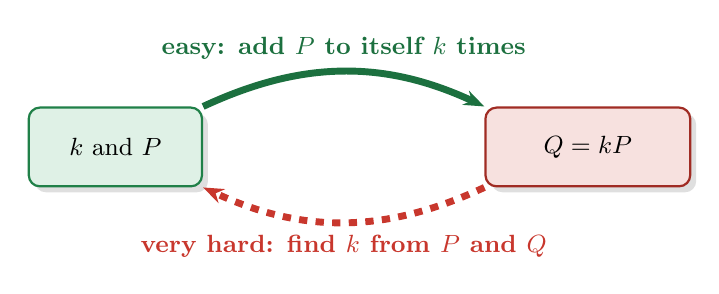
\begin{tikzpicture}
    \node[box=leaf,minimum width=22mm,minimum height=10mm] (k) at (0,0) {$k$ and $P$};
    \node[box=brick,minimum width=26mm,minimum height=10mm] (q) at (6,0) {$Q = kP$};
    \draw[->,leaf!70!black,line width=2.5pt] (k.north east) to[bend left=25] node[above,font=\small\bfseries]{easy: add $P$ to itself $k$ times} (q.north west);
    \draw[->,brick,line width=2.5pt,dashed] (q.south west) to[bend left=25] node[below,font=\small\bfseries]{very hard: find $k$ from $P$ and $Q$} (k.south east);
  \end{tikzpicture}
  \vspace{5mm}
  \begin{columns}[T]
    \begin{column}{0.48\textwidth}
      \begin{block}{Elliptic curve discrete logarithm}
        \small $kP$ means $P + P + \dots + P$ ($k$ times). Using doubling, it can be computed quickly even for huge $k$.
      \end{block}
    \end{column}
    \begin{column}{0.48\textwidth}
      \begin{alertblock}{Why it is strong}
        \small Finding $k$ is \textbf{harder} than ordinary discrete logs or factoring of the same size, which is why ECC keys can be so short.
      \end{alertblock}
    \end{column}
  \end{columns}
\end{frame}

% ------------------------------------------------------------
\begin{frame}{ECC Diffie--Hellman Key Exchange}
  \centering
  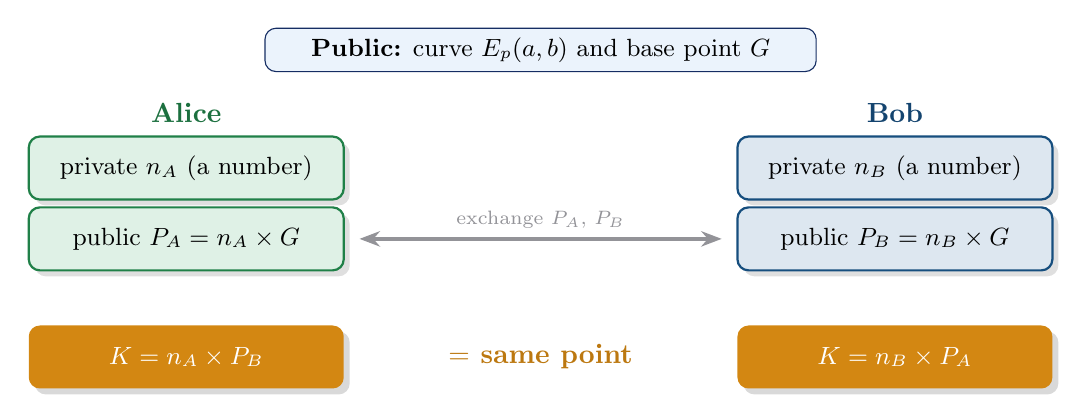
\begin{tikzpicture}
    \node[fill=sky,draw=navy,rounded corners,font=\small,minimum width=70mm] at (4.5,1.5) {\textbf{Public:} curve $E_p(a,b)$ and base point $G$};
    \foreach \l/\x/\c/\s/\pub/\k in {Alice/0/leaf/n_A/P_A = n_A \times G/K = n_A \times P_B,Bob/9/ocean/n_B/P_B = n_B \times G/K = n_B \times P_A}{
      \node[font=\bfseries,text=\c!70!black] at (\x,0.7) {\l};
      \node[box=\c,minimum width=40mm,font=\small] at (\x,0) {private $\s$ (a number)};
      \node[box=\c,minimum width=40mm,font=\small] at (\x,-0.9) {public $\pub$};
      \node[solid box=amber!90!black,minimum width=40mm,font=\small] at (\x,-2.4) {$\k$};
    }
    \draw[<->,very thick,ink!50] (2.2,-0.9) -- node[above,font=\scriptsize]{exchange $P_A$, $P_B$} (6.8,-0.9);
    \node[font=\bfseries,text=amber!80!black] at (4.5,-2.4) {$=$ same point};
  \end{tikzpicture}
  \vspace{3mm}
  \begin{block}{Why the keys match}
    \small $n_A \times P_B = n_A \times n_B \times G = n_B \times P_A$. Just like ordinary Diffie--Hellman, but with point multiplication instead of exponentiation.
  \end{block}
\end{frame}

% ------------------------------------------------------------
\begin{frame}{ECC Encryption and Decryption}
  \begin{columns}[c]
    \begin{column}{0.52\textwidth}
      \centering
      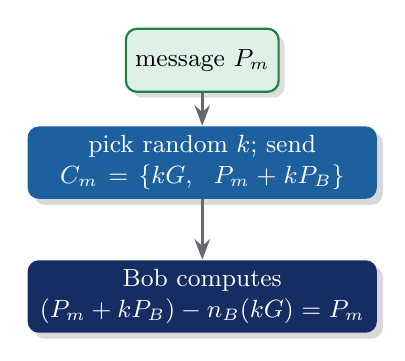
\begin{tikzpicture}
        \node[box=leaf,minimum width=18mm] (pm) at (0,0) {message $P_m$};
        \node[solid box=ocean,minimum width=44mm,font=\small,text width=42mm,align=center] (e) at (0,-1.3) {pick random $k$; send\\$C_m = \{kG,\ \ P_m + kP_B\}$};
        \node[solid box=navy,minimum width=44mm,font=\small,text width=42mm,align=center] (d) at (0,-3.0) {Bob computes\\$(P_m + kP_B) - n_B(kG) = P_m$};
        \draw[flow] (pm) -- (e); \draw[flow] (e) -- (d);
      \end{tikzpicture}
    \end{column}
    \begin{column}{0.46\textwidth}
      \begin{enumerate}\small\setlength{\itemsep}{3pt}
        \item The message is encoded as a \textbf{point} $P_m$ on the curve
        \item Alice picks a random $k$ and sends two points
        \item Bob multiplies $kG$ by his private key $n_B$ and subtracts
      \end{enumerate}
      \begin{exampleblock}{Why it works}
        \small $n_B(kG) = k(n_B G) = kP_B$, so subtracting it removes the ``mask'' and leaves $P_m$.
      \end{exampleblock}
      {\small An attacker would need $k$ from $kG$: the hard problem.}
    \end{column}
  \end{columns}
\end{frame}

% ------------------------------------------------------------
\begin{frame}{Comparing RSA, Diffie--Hellman and ECC}
  \centering
  \renewcommand{\arraystretch}{1.45}
  \small
  \begin{tabular}{>{\bfseries}l >{\columncolor{brick!8}}c >{\columncolor{amber!10}}c >{\columncolor{leaf!10}}c}
    \toprule
    \rowcolor{navy}\textcolor{white}{Feature} & \textcolor{white}{\textbf{RSA}} & \textcolor{white}{\textbf{Diffie--Hellman}} & \textcolor{white}{\textbf{ECC}}\\
    \midrule
    Hard problem & Factoring & Discrete log & EC discrete log\\
    Uses & Enc, sign, key exch. & Key exchange & Enc, sign, key exch.\\
    Key size for 128-bit security & 3072 bits & 3072 bits & 256 bits\\
    Speed & Slow & Slow & Faster\\
    Best for & General use, web & Agreeing on keys & Phones, smart cards\\
    \bottomrule
  \end{tabular}
\end{frame}

% ------------------------------------------------------------
\begin{frame}{Quick Check}
  \centering
  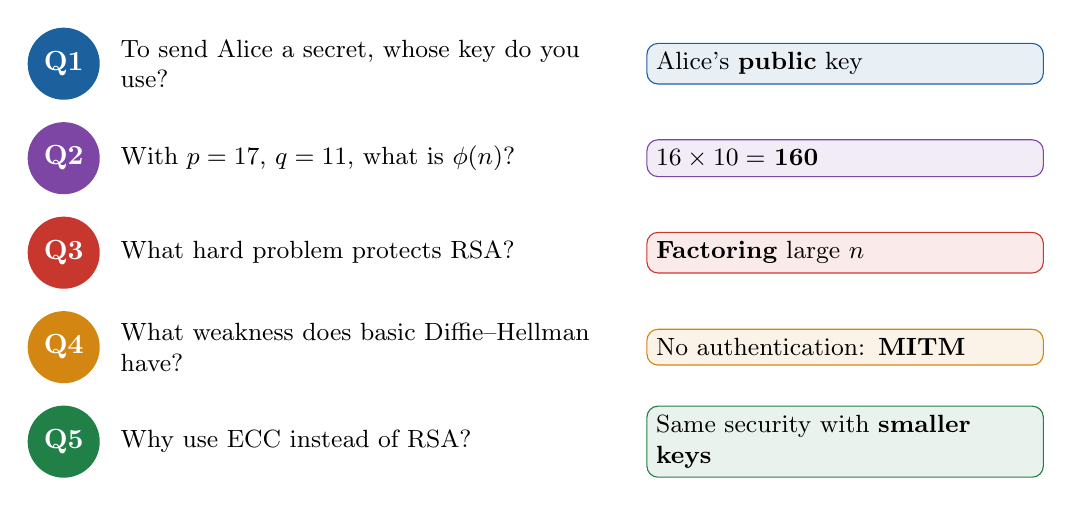
\begin{tikzpicture}
    \foreach \q/\a/\c [count=\i] in {
      To send Alice a secret\comma{} whose key do you use?/Alice's \textbf{public} key/ocean,
      With $p = 17$\comma{} $q = 11$\comma{} what is $\phi(n)$?/$16 \times 10 = $ \textbf{160}/grape,
      What hard problem protects RSA?/\textbf{Factoring} large $n$/brick,
      What weakness does basic Diffie--Hellman have?/No authentication: \textbf{MITM}/amber!90!black,
      Why use ECC instead of RSA?/Same security with \textbf{smaller keys}/leaf!80!black}
    {
      \node[circle,fill=\c,text=white,font=\bfseries,minimum size=8mm] (n\i) at (0,-\i*1.2) {Q\i};
      \node[anchor=west,font=\small,text width=60mm] at (0.6,-\i*1.2) {\q};
      \node[anchor=west,fill=\c!10,draw=\c,rounded corners,font=\small,text width=48mm] at (7.4,-\i*1.2) {\a};
    }
  \end{tikzpicture}
\end{frame}

% ------------------------------------------------------------
\begin{frame}{Module 8 Summary}
  \begin{columns}[T]
    \begin{column}{0.32\textwidth}
      \begin{block}{Lesson 11: Public Key}
        \scriptsize
        \begin{itemize}\setlength{\itemsep}{0pt}
          \item Key pair: public + private
          \item Confidentiality and signatures
          \item Enc/dec, signature, key exchange
          \item Requirements; trap-door functions
          \item Cryptanalysis
        \end{itemize}
      \end{block}
    \end{column}
    \begin{column}{0.32\textwidth}
      \begin{alertblock}{Lesson 17: RSA \& DH}
        \scriptsize
        \begin{itemize}\setlength{\itemsep}{0pt}
          \item RSA keys, $C = M^e$, $M = C^d$
          \item Square-and-multiply; CRT
          \item Five attacks; factoring
          \item Diffie--Hellman key exchange
          \item Man-in-the-middle attack
        \end{itemize}
      \end{alertblock}
    \end{column}
    \begin{column}{0.32\textwidth}
      \begin{exampleblock}{Lesson 19: ECC}
        \scriptsize
        \begin{itemize}\setlength{\itemsep}{0pt}
          \item $y^2 = x^3 + ax + b$
          \item Point addition and doubling
          \item Curves mod $p$
          \item $Q = kP$ hard problem
          \item ECC key exchange, encryption
        \end{itemize}
      \end{exampleblock}
    \end{column}
  \end{columns}
  \vspace{2mm}
  \begin{alertblock}{Review questions}
    \small
    1.~Explain the principles of public-key cryptosystems. \quad 2.~Explain the RSA algorithm with an example. \quad
    3.~Explain Diffie--Hellman key exchange and the man-in-the-middle attack. \quad 4.~Explain elliptic curve cryptography.
  \end{alertblock}
\end{frame}

% ------------------------------------------------------------
\begin{frame}{References}
  \begin{enumerate}\setlength{\itemsep}{8pt}
    \item William Stallings, \emph{Cryptography and Network Security}, PHI Publishers.
    \item Charlie Kaufman, Radia Perlman, \emph{Network Security}, Pearson Education.
    \item Bruce Schneier, \emph{Applied Cryptography}, John Wiley \& Sons.
    \item Roberta Bragg, \emph{Network Security: The Complete Reference}, TMH.
  \end{enumerate}
  \vspace{6mm}
  \centering
  
\begin{tikzpicture}
    \node[fill=navy,text=white,rounded corners=8pt,inner sep=10pt,font=\Large\bfseries,drop shadow] {Thank You! \; Questions?};
  \end{tikzpicture}
\end{frame}

\end{document}
